%### IEEE ###
\documentclass[conference]{IEEEtran}
  % Use this line for a4 paper
%\IEEEoverridecommandlockouts
  % Needed if you want to use the \thanks command
%\overrideIEEEmargins
  % Needed to meet printer requirements.
 
\usepackage{algorithm}
\usepackage{algorithmic}
	
\usepackage{amsmath}
\usepackage{amsfonts}
	
\usepackage{graphics}
\usepackage{graphicx}
%\usepackage[lined,boxed,commentsnumbered]{algorithm2e}

%\usepackage{hyperref}
\usepackage{verbatim}

\renewcommand{\L}{\mathcal{L}}

\usepackage{color}
\newcommand{\todo}[1]{{\small\color{red}[#1]}}

%CHEAT CODES
\renewcommand{\baselinestretch}{.987}
\renewcommand{\textfloatsep}{0.88ex}


\begin{document}

% can use linebreaks \\ within to get better formatting as desired
\title{Robot Learning Simultaneously a Task and \\ How to Interpret Human Instructions}


% author names and affiliations
% use a multiple column layout for up to three different
% affiliations
\author{
\IEEEauthorblockN{Jonathan Grizou}
\IEEEauthorblockA{Flowers Team\\
 INRIA / ENSTA-Paristech\\
France\\
jonathan.grizou@inria.fr}
\and
\IEEEauthorblockN{Manuel Lopes}
\IEEEauthorblockA{Flowers Team\\
INRIA / ENSTA-Paristech\\
France\\
manuel.lopes@inria.fr}
\and
\IEEEauthorblockN{Pierre-Yves Oudeyer}
\IEEEauthorblockA{Flowers Team\\
INRIA / ENSTA-Paristech\\
France\\
pierre-yves.oudeyer@inria.fr}
}


%\thanks{The authors are with the Flowers Team, an INRIA and ENSTA-Paristech joint-lab. Work (partially) supported by INRIA, Conseil R\'egional d'Aquitaine and the ERC grant EXPLORERS 24007.}}


\maketitle

\begin{abstract}
This paper presents an algorithm to bootstrap shared understanding in a human-robot interaction scenario where the user teaches a robot a new task using teaching instructions yet unknown to it. In such cases, the robot needs to estimate simultaneously what the task is and the associated meaning of instructions received from the user. For this work, we consider a scenario where a human teacher uses initially unknown spoken words, whose associated unknown meaning is either a feedback (good/bad) or a guidance (go left, right, ...). We present computational results, within an inverse reinforcement learning framework, showing that a) it is possible to learn the meaning of unknown and noisy teaching instructions, as well as a new task at the same time, b) it is possible to reuse the acquired knowledge about instructions for learning new tasks, and c) even if the robot initially knows some of the instructions' meanings, the use of extra unknown teaching instructions improves learning efficiency.
\end{abstract}
\maketitle
\section{Introduction}
\label{sec:Introduction}

Robots are becoming increasingly important, targeting human assistance at home or at the workplace. Yet, such robots can not be pre-programmed to face every day problems in our open ended and dynamic environments. This challenge requires to develop learning algorithm for the robot to adapt to its environment. Among other forms of adaptation to the environment, \textit{social learning}, where knowledge is transmitted from humans to robots through social interaction, is of primordial importance. It has the advantage of being an intuitive way for humans to instruct robots. A usual assumption in such systems is that the learner and the teacher share a mutual understanding of the meaning of each others' signals, and in particular the robot is usually assumed to know how to interpret teaching instructions from the human. In practice, the range of accepted instructions is limited to the one predifined by the system developer. However non-expert users might have very different preferences and predefined instructions might not be well accepted. We believe that robots should themselves be able to adapt progressively to every user's particular teaching behaviors at the same time as they learn new skills. %The aim of this work is to make a first step in this direction.
%in order for a robot to learn from a human user, it must be possible for humans to communicate their intentions and preferences to such machines. 

Research in robotics has long been inspired by human social learning. Among other aspects, learning by demonstration/imitation has attracted most attention. It has provided several examples of efficient learning in robotic systems \cite{Argall09lfdsurvey}\cite{lopes10imitationchapter}. Data from a human teacher has been used as initial condition for further self-exploration in robotics \cite{nicolescu2003natural}, bootstrapping further intrinsically motivated learning \cite{nguyen2011bootstrapping}, information about the task solution \cite{Calinon07}, information about the task representation \cite{macl07affimit}, among others. Several representations have been used to generalize the demonstration data using reinforcement learning \cite{Thomaz2008}, inverse reinforcement learning \cite{macl07affimit}\cite{Abbeel04icml}, or regression methods \cite{Calinon07}\cite{chernova09jair}. The different formalisms make use of various kinds of information and extract different knowledge, either direct policy information or a reward function that explains the behavior.
%
\begin{figure}[!t]
	\begin{center}
   		%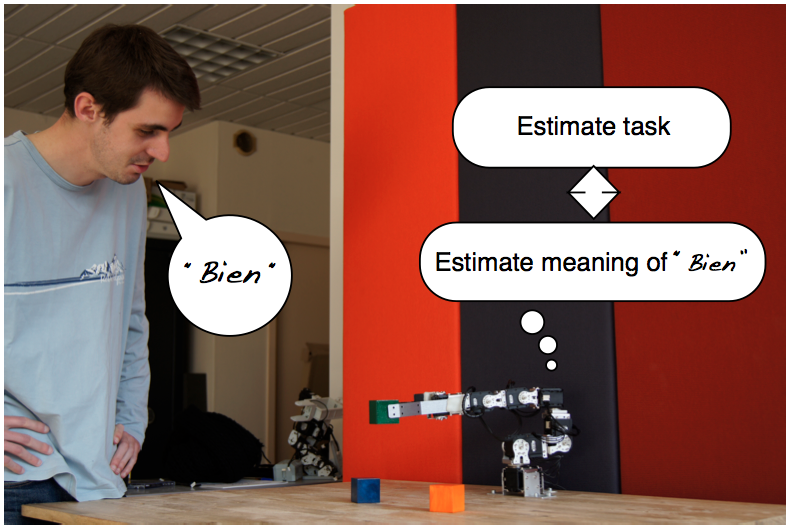
\includegraphics[width=0.8\columnwidth]{images/exp2.png}
   		%\caption{A human teacher is interacting with a robot using spoken language. The provided teaching signals allow the robot, which does not know before hand their associated meanings, to estimate simultaneously what the task is and the meaning of the spoken words.}
   		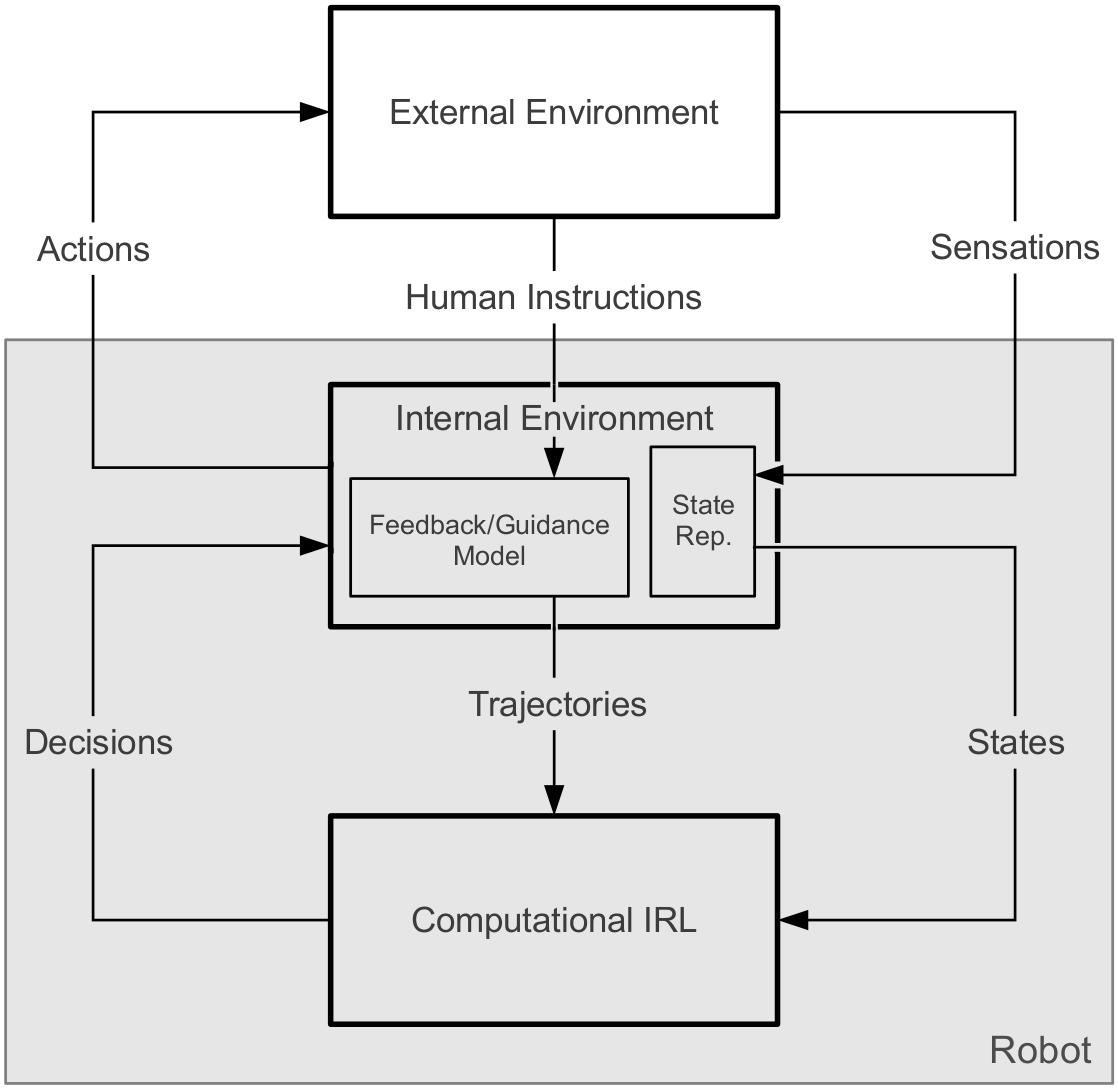
\includegraphics[width=0.8\columnwidth]{images/problem_representation.png}
   		\caption{Reinforcement learning oriented architecture of our problem. Humans provide instructions for learning a task whose meanings are a priori unknown. Thus, the meaning of these instructions has to be learnt by the robot in addition to learning the task itself.}
		\label{fig1} 
   \end{center}
\end{figure}

For most of those systems, the human demonstrations are provided in a batch perspective where data acquisition is done before the learning phase. Recently it has been suggested that \textit{interactive learning} \cite{nicolescu2003natural}\cite{Breazeal2004} might be a new perspective on robot learning, that combines the ideas of learning by demonstration, learning by exploration and tutor feedback. Under this approach the teacher interacts with the robot and provides extra feedback or guidance. In addition, the robot can act to improve its learning efficiency. Approaches have considered: extra reinforcement signals \cite{Thomaz2008}, action requests \cite{macl09airl}, disambiguation among actions \cite{chernova09jair}, preferences among states \cite{Mason2011}, iterations between practice and user feedback sessions \cite{judah2010rlandcritique}, and choosing actions that maximize the user feedback \cite{knox2009interactively}. %In \cite{Cakmak2010a} the authors compare the results when the robot has the option of asking or not the teacher for feedback, and in \cite{cakmak2012designing} study what it means for a robot learner to ask good questions.

An important challenge for such interactive systems is to deal with nonexpert humans. Several studies discuss the various behaviors naive teachers use when instructing robots \cite{Thomaz2008,Cakmak2010}. An important aspect is that the feedback is frequently ambiguous and deviates from the mathematical interpretation of a reward; or a sample trajectory deviates from an optimal policy. For instance, in the work of \cite{Thomaz2008} the teachers frequently gave a positive reward for exploratory actions even if the signal was used by the learner as a standard reward. Also, even if we can define an optimal teaching sequence, humans do not necessarily behave according to those strategies \cite{Cakmak2010}.

In addition, users may have various expectations and preferences when interacting with a robot; therefore predifined protocols or teaching signals may bother the user and dramatically decrease the performance of the learning system \cite{rouanet2013impact}. In this paper, we present an algorithm allowing a robot to learn the meaning of human teaching instructions in the process of learning a task (as illustrated in figure~\ref{fig1}). Importantly, the system does not need bootstraping with known instructions, but only requires knowledge about the possible structures of meanings and tasks. The learnt instruction-to-meaning association can then be reused in the learning of novel tasks, progressively increasing the knowledge of the robot. We will also show that, by combining known and unknown teaching signals, the robot is able to take advantages of unknown instructions to learn more efficiently than by relying only on known ones. We do not claim that we should not rely on predefined signals but rather that the feedback or guidance provided through predefined protocols could be completed with the particular teaching signals that each user provides.

We extend the work presented in \cite{macl11simul}, which introduced a preliminary approach to this problem considering an abstract symbolic space of instructions in simulation. Here, we allow the robot to learn the meaning of unknown instructions without the need of bootstrapping the system with known instructions and by considering real natural speech waves data instead of symbolic labels, as well as a physical human-robot interaction scenario. In \cite{heckmann2009teaching}, the robot ASIMO is taught to associate new spoken signals to visual object properties, both in noisy conditions and without the need for bootstrapping. However the robot is not learning a sequential task but correlations between clusters in speech and visual spaces. Similarly Kindermans et al. \cite{Kindermans2012a} proposed an unsupervised training of a P300-based BCI systems using application constraints. Their formalism is close to the one described in this paper; however, our system is able to provide a confidence about its current knowledge of the task and instruction-to-meaning association.

Our algorithm differs from typical learning by demonstration systems because data is acquired in an interactive and online setting. It improves from previous learning by interaction systems in the sense that the instructions received are continuous unlabelled signals. Our framework is generic and the signals provided by the teacher can be gestures, facial expression, or any modalities as long as we can project them into a fixed length continuous representation.

%; and that they form differentiable clusters in such space. In addition, the algorithm is able to recover from teaching mistake, i.e. when the user send an inappropriate signals to the robot (e.g. saying \textit{'Correct'} instead of \textit{'Wrong'}).

Our contribution is threefold: a) we provide an online learning algorithm which makes it possible to learn the meaning of unknown and noisy instructions, as well as a new task at the same time, b) we enable the reuse of acquired knowledge about instructions for learning new tasks, and c) in the case where the robot initially knows some of the instructions meanings, extra unknown teaching signals are used to improve learning efficiency.

In Section~\ref{sec:Algorithm}, we will provide details on the algorithm. % which is general and does not make particular assumptions on how the task or the instructions are represented. 
The following sections present an application of this algorithm to a particular interaction scenario. We will introduce first the robotic system, the interaction protocol and the signals processing unit. Finally, we will present results from both simulations and an experiment with a real robot.


%Concretely the robot can learn a task from isolated words in any languages or sounds such as hand clapping (e.g. the user could use the word \textit{``Dog''} to mean \textit{``Correct''}). In addition the user is free to teach any task (from a set of possible one) to the robot. Both task and speech signals to meanings association are learnt simultaneously, meaning that no previous user specific training are needed. However the interaction protocol is constrained to be turn taking and possible signals meanings are reduced to feedback or guidance on the robot's actions.







\section{Algorithm}
\label{sec:Algorithm}

In this section, we present our computational model by considering the following cases: 1) feedback instructions 2) guidance instructions, and 3) how to include known sources of instructions

Our goal is to learn simultaneously a task $\xi$ and the meaning of the instructions $n$ provided by the user. We assume such instructions are represented in a fixed length feature vector with continuous values that are generated from a probabilistic model. For each particular task $\xi$ we only assume that we are able to compute a policy $\pi$, which represents the probability of choosing a given action $a$ in a given state $s$, $\pi^{\xi}(s,a)=p(a|s,\xi)$.
%for a particular task $\xi$ we are able to compute its corresponding policy $\pi$, which represents the probability of choosing a given action $a$ in a given state $s$, $\pi^{\xi}(s,a)=p(a|s,\xi)$.
We consider that the human-robot interaction sessions give data in the form $\{(s_i,a_i,n_i),\ i = 1,\ldots,m\}$, i.e. a sequence of states, actions and teaching signals triplets. At each iteration the robot performs one action and waits for the instruction from the teacher.
%It is important to note that the teaching signal is provided only after the sequence ${s,a,s'}$ has been observed by the teacher. The problem of temporal assignement is not considered here and will be solved in pratice by the use of a contolled protocol.
%
%Our goal is to simultaneously find a set of parameters $\theta$ and $\xi$ that represents both the associated meaning of the teaching signals and the task that the user is teaching. We present the algorithm in two parts: first we assume the task is known ($\xi$) and then we show how to learn the task and the signal meanings simultaneously.
%
%If $n_i$ is a feedback signal, it is related to the optimality of choosing action $a_i$ in state $s_i$. If $n_i$ is a guidance signal, it is related to the optimal action to choose in state $s_{i+1}$. 
%
\subsection{Learning the Instructions Meaning}
%
We start by assuming that the teacher provides a simple binary feedback whose meaning $f$ can be in $F=\{\texttt{correct},\texttt{wrong}\}$. For each feedback, the user produces a signal in natural language that might be a corresponding word (e.g. \textit{``ok'', ``good'', ``bad'', ``wrong''}). In this first step we want to learn the parameters $\theta$ of the signal production model:
% 
\begin{equation}
\theta^* = \arg\max_\theta~p(n|s,a,\xi,\theta)
\label{eq:initprob}
\end{equation}
%
This model is very difficult to identify but if we would have access to an hidden variable $z$, representing the meaning of the instruction that the user said, it would be simplified and represented as $p(n|z,\theta)$ where $n$ is the signal observed. This meaning is generated according to the following model $p(z|s,a,\xi)=p(z|f)p(f|s,a,\xi)$ where $p(f|s,a,\xi)$ represents the ideal feedback for task $\xi$ when the teacher observes action $a$ in state $s$, and $p(z|f)$ consider what the user actually provided as feedback, considering the way he likes to provide it and also the mistakes he makes. The component $p(f|s,a,\xi)$ is fixed and derives directly from the task representation used. We do not assume any particular structure for $p(z|f)$ and even allow it to be different for each sample. This allows for a larger variety of teacher behaviors including the statistics of errors made on the instructions. Due to these reasons, and without lack of generality we will always refer to $p(z|s,a,\xi)$.

Due to the uncertainty in the expected meaning $z$, the task model $\xi$, variability in the feedback signals $n$ (e.g. words are never pronounced the same way) and occasional teaching mistakes, we are not sure if each instruction produced by the teacher corresponds to the meaning \texttt{correct} or \texttt{wrong}. As we are in the presence of a hidden information problem we will rely on an \textit{Expectation-Maximization algorithm} (EM) to solve the problem in Eq.~\ref{eq:initprob}.

We start by defining the complete likelihood model:
%
\begin{eqnarray}
\L(\theta,\xi) &=&  p(n|s,a,\xi,\theta)\nonumber\\
			   %&=&  \prod_{i} p(n_i | s_i, a_i, \xi, \theta)\nonumber\\
			   &=& \prod_{i} \L_{i}(\theta,\xi)\nonumber
\end{eqnarray}			
with
\begin{eqnarray}
\L_i(\theta,\xi) &=&  p(n_i|s_i,a_i,\xi,\theta)\nonumber\\
				&=&	\sum_{j \in F} p(n_i|z = j,s_i,a_i,\xi,\theta)~p(z = j|s_i,a_i,\xi,\theta)	\nonumber\\
				&=&	\sum_{j \in F} \underbrace{p(n_i|z = j,\theta)}_{\text{instruction}}~\underbrace{p(z = j|s_i,a_i,\xi)}_{\text{meaning}}	\nonumber\\
				&=&	\sum_{j \in F} p(n_i|z = j,\theta)~z_{ij}^{\xi}
				\label{eq:lik}
\end{eqnarray}

%\begin{eqnarray}
%\L_i &=&  p(n_i|s_i,a_i,\xi,\theta)\nonumber\\
%				&=&	\sum_{j \in F} p(n_i|z = j,s_i,a_i,\xi,\theta)~p(z = j|s_i,a_i,\xi,\theta)	\nonumber\\
%				&=&	\sum_{j \in F} \underbrace{p(n_i|z = j,\theta)}_{\text{instruction}}~\underbrace{p(z = j|s_i,a_i,\xi)}_{\text{meaning}}	\nonumber\\
%				&=&	\sum_{j \in F} p(n_i|z = j,\theta)~z_{ij}^{\xi}
%				\label{eq:lik}
%\end{eqnarray}
%
with $z_{ij}^{\xi} = p(z = j|s_i,a_i,\xi)$. Where in the second step we introduce the hidden variable $z$ as described earlier. The meaning $z$ depends only on the state-action pair $(s,a)$ evaluated in the scope of the task $\xi$. The instruction $n$ depends solely on the signal generation model, parameterized by $\theta$, corresponding to the meaning (i.e. the class) $z$. The ML estimate of $\theta$ is found by maximizing $\log{\L}$. We first perform the \textit{expectation} step by defining the $F(\theta|\theta^t)$ function for a given task $\xi$:
%
%\begin{eqnarray}
%	F(\theta|\theta^t) &=& \sum_{ij} \log{(\L_i)}~p(z_i=j|n_i,s_i,a_i,\xi,\theta^t)\nonumber\\
%					&=& \sum_{ij} \left(\log{p(n_i|z_i,\theta)}+\log{z_i^{\xi}}\right) w_{ij}
%					\label{eq:F}
%\end{eqnarray}
\begin{eqnarray}
F(\theta|\theta^t) &=& \mathbb{E}[\log{\L(\theta)}| n, s, a, \xi, \theta^t]\nonumber\\
                   &=& \sum_i \sum_{j \in F} \log{\L_{ij}(\theta)}~p(z=j|n_i,s_i,a_i,\xi,\theta^t)\nonumber\\
                   &=& \sum_i \sum_{j \in F} \left(\log{p(n_i|z=j,\theta)}+\log{z_{ij}^{\xi}}\right) w_{ij}
					\label{eq:F}
\end{eqnarray}
%
with
\begin{eqnarray*}
 w_{ij} &=& p(z=j|n_i,s_i,a_i,\xi,\theta^t)\\
        &\propto& p(n_i|z=j,s_i,a_i,\xi,\theta^t)~p(z=j|s_i,a_i,\xi,\theta^t)\\
		&=& p(n_i|z=j,\theta^t)~p(z=j|s_i,a_i,\xi)\\
\end{eqnarray*}
%
The \textit{M-step} is the maximization of Eq.~\ref{eq:F}:
%
\begin{equation}
\theta^{t+1} = \arg\max_{\theta} F(\theta|\theta^t) 
\label{eq:m-step}
\end{equation}
%
This step depends on the specific statistical models we use for the instruction learning, i.e. the classifier. If they are modeled as gaussian distributions then the usual equations for a gaussian mixture hold and we can solve the maximization problem analytically. As for more complex interactions the instructions produced by the teacher will be more complex we will also try learning algorithm with a higher capacity, e.g. \textit{SVMs}. If such classifier is not able to use probabilistic labels, we approximate Eq.~\ref{eq:F} with a hard threshold for $z_{ij}^{\xi}$ and train the SVM on the corresponding dataset. The full process is summarized in Algorithm \ref{alg:simpleem}.
%
\begin{algorithm}
\caption{EM for learning Instructions Meaning}
\begin{algorithmic}[1]
\REQUIRE Data $\{(s_i,a_i,n_i),\ i = 1,\ldots,m\}$
\REQUIRE Task $\xi$
\WHILE{\TRUE} 
\STATE E-Step \\ $F(\theta|\theta^t) = \sum_{ij} \left(\log{p(n_i|z=j,\theta)}+\log{z_{ij}^\xi}\right) w_{ij}$ \\
$w_{ij} = p(n_i|z=j,\theta^t)~p(z=j|s_i,a_i,\xi)$
\STATE M-Step \\ $\theta^{t+1} = \arg\max_{\theta} F(\theta|\theta^t)$
\ENDWHILE
\end{algorithmic}
\label{alg:simpleem}
\end{algorithm}

\subsection{The guidance case}

The version presented above is well suited to learn instructions that correspond to \texttt{correct} or \texttt{wrong}. We can devise another interaction scheme where the teacher provides the names of actions to be done and the robot has to learn which action do each instruction corresponds to. We can see these instructions as a guidance signal or a voice operated remote control. We can deal with this situation by redefining the meaning of $z$. Now this variable indicates the name of the optimal action in state $s$ according to task $\xi$. We define $G$ as the set of guidance meanings, i.e. the name of the possible action. Under this new definition we can change the likelihood function to:
%
\begin{eqnarray}
\L_{i}(\theta,\xi) &=&  p(n_i|s_i,a_i,\xi,\theta)\nonumber\\
				&=&	\sum_{j \in G} p(n_i|z = j,\theta)~p(z = j|s_i,\xi)	\nonumber\\
				&=&	\sum_{j \in G} p(n_i|z = j,\theta)~z_{ij}^{\xi}
				\label{eq:likact}
\end{eqnarray}
%
with $z_{ij}^{\xi} = p(z = j|s_i,\xi)$ and where we dropped the dependence on the action.

\subsection{Learning Simultaneously a Task and Instructions Meaning}

We now relax the assumption that we have an estimation of what the task is: we consider that the learner is able to sample tasks from a finite set according to a given distribution. The goal is to find, from this distribution, the task $\xi^*$ that is closer to the one the user is teaching to the robot. At each iteration the algorithm evaluates the likelihood of every task hypothesis. For this, it needs to apply Algorithm \ref{alg:simpleem} for every task hypothesis. The global process of simultaneously estimating the task and the instruction model is shown in Algorithm \ref{alg:interlearn}.

\begin{algorithm}
\caption{Learning Simultaneously a Task and Instructions Meaning}
\begin{algorithmic}[1]
%\REQUIRE Set of $m$ possible actions $A$ 
%\REQUIRE Set of $n$ possible states $S$
%\STATE Sample $l$ different tasks $\xi_1,\ldots,\xi_l$
\REQUIRE Set of $l$ different tasks hypothesis $\xi_1,\ldots,\xi_l$
\STATE $i = 1$
\STATE $s_1 \leftarrow$ current state
\WHILE{\TRUE} 
	\STATE Choose and apply action $a_i$
	\STATE Observe next state $s_{i+1}$ and user instructions $n_i$
	\FORALL{$k=1,\ldots,l$}		
		\STATE From Algorithm \ref{alg:simpleem} find:\\
		$\theta_k = \arg\max_{\theta} F(\theta|\theta^0, \xi_k)$\\
		$q_k(\xi_k) = \L(\theta_k, \xi_k)$
	\ENDFOR
	%\STATE $\xi^*=\arg\max_k \L(\theta_k(\xi_k))$
	\STATE Resample $\xi_k$, $k = 1,\ldots,l$ according to $q_k(\xi_k)$	
	\STATE $i \leftarrow i+1$
\ENDWHILE
\RETURN $q_k(\xi_k),\ \xi_k,\  k = 1,\ldots,l $
\end{algorithmic}
\label{alg:interlearn}
\end{algorithm}

We are now simultaneously solving two optimization problems. We are trying to select the best task hypothesis and the best instruction-to-meaning mapping. We have to rely on an approximation to avoid the computation of all possible pairs of tasks and meaning models. To do so we first optimize the meaning model for each task hypothesis using Alg. \ref{alg:simpleem}. Then, for the list of possible tasks we compute the likelihood of the observed data to give us the posterior distribution of tasks. As there might be no feasible task, we have to use the noiseless version of the feedback model as the likelihood in Step 7 of Alg. \ref{alg:interlearn}.

An intuition on how the algorithm works is to imagine the agent assigning hypothetic labels (i.e. meanings) to instructions for each task of the distribution. The agent is updating as many models as task hypothesis and is looking for the one from which emerges a coherence in the interpretation of the instructions. Here, we are assuming that if the correct labels are known, signals of same meaning (e.g. utterances of the same word) can be identified with good accuracy using the chosen classifier parameterized by $\theta$. % Such structure is estimated ($\L_i$) based on the performance of a classifier parameterized by $\theta$. 
In case of a gaussian classifier, $\theta$ represents the mean and covariance of each class. The algorithm will start failing if signals used for different meanings cannot be differentiated by the classifier, or if the classifier is overfitting the data.

%The main difficulty of simultaneously learning both task and teaching signals is the existence of local minima in the sense that for different tasks the same signals could be interpreted in different ways. Consider for instance the case of a Nx1 grid world, where the agent has to learn to reach the leftmost state. Note that, in this specific case, if we change the correct to incorrect feedback in all the states, it is possible to find another task, e.g. going to the rightmost state, that verifies the conditions in all states. This particular property between hypothesis is called symmetry. Our algorithm can not differentiate fully symmetric tasks. However it is always possible to break the symmetry, in our example by adding a ``stop'' action that is valid only at the goal state.

The computational complexity of the algorithm grows linearly with the number of possible hypothesis and with the number of data-points. Even with such a low complexity, for some problems the number of possible hypothesis might be very large. The complexity of this algorithm can be reduced in two ways. First we can consider a reduced set of task hypothesis and apply a resample step according to the estimated likelihoods, as shown in Step 10. Another way to reduce the complexity is to consider that the dataset does not cover the whole state-space. Because of this, Step 7 does not need to be applied to all hypothesis but only to the equivalence classes of the policies induced by the hypothesis set according to the dataset.

\subsection{Including prior knowledge}

Although we took such a difficult challenge of learning without assuming knowledge of the instructions, for a practical case, it is more reasonable to combine pre-specified instructions with an adaptation to new ones. For instance, the robot might be equipped with a console with a simple interface such as a green and a red button corresponding to correct and incorrect feedback and we want to combine this information with unknown sources of instructions.
%Such known source of information may help the agent learning the task and infering the meaning of received instruction.

The use of those extra sources of information is straightforward in our statistical formalism: we can change the likelihood model from Eq.~\ref{eq:lik} and extend the model $p(z|s,a,\xi)$ with an observed variable $d$ representing the noisy (in terms of teaching mistakes) but known feedback. The model becomes:
%
\begin{eqnarray}
\L_{i}(\theta, \xi) &=&  p(n_i,d_i|s_i,a_i,\xi,\theta)\nonumber\\
				&=&	\sum_{j} p(n_i|z = j,\theta)~p(d_i|z = j)~p(z = j|s_i,a_i,\xi)\nonumber\\
				\label{eq:lik2}
\end{eqnarray}
%
In this way we still accept that the human does not use the pre-define interface or that it makes mistakes. In the former case we just assume $p(d|z)=1$ and we recover the original likelihood function, in the latter the complete rule will take the noise into account. Identically, if the user does not provide any known instructions, we just assume $p(n|z,\theta)=1$.


\begin{comment}
\section{Algorithm}
\label{sec:Algorithm}

Our goal is to learn simultaneously a task $\xi$ and the meaning of the teaching signals $n$ provided by the user.  %Contrary to other approaches (e.g. \cite{macl11simul}) we are interested in the case where the signals are real social signals, in particular real speech like in the presented experiments, but this could also be gestures or facial expressions. 
We assume such signals are represented in a fixed length feature vector and are generated from a probabilistic model $p(n|z,\theta)$ where $n$ is the signal observed, $z$ is the meaning of the signal among a pre-defined set of possible meanings and $\theta$ are the parameters of this model.

We do not make particular assumptions on how the task is represented and just assume that for a particular task $\xi$ we are able to compute a policy $\pi$ which represents, for a given task $\xi$, the probability of choosing a given action $a$ in a given state $s$, $\pi^{\xi}(s,a)=p(a|s,\xi)$. We also assume that we have a model of the teaching protocol that gives us the probability of receiving a given feedback $z$ from a user $p(z|s,a,\xi)$. We further assume that from a human-robot interaction session we acquire data in the form $\{(s_i,a_i,n_i),\ i = 1,\ldots,m\}$, i.e. a sequence of states, actions and teaching signals sounds triplets. The problem of temporal assignement is not considered here and will be solved in pratice by the use of a contolled protocol.

Our goal is to simultaneously find a set of parameters $\theta$ and $\xi$ that represents both the utterances of the user and the task that the user is teaching. We present the algorithm in two parts: first we assume that we have an estimation of what the task might be $\xi$ and then we show how to learn the task and the signal meanings simultaneously.

\subsection{Learning the teaching signals}
\label{sec:learnfeed}

We start by assuming that the teacher provides a simple binary feedback which meaning can be either \texttt{correct} or \texttt{wrong}. For each feedback, the user produces a signal in natural language that might be a corresponding word (e.g. \textit{``ok'', ``correct'', ``good'', ``bad'', ``wrong''}, or any other word, or even an interjection). In this first step we want to learn the parameters $\theta$ of the signal production model:
 
\begin{equation}
\theta = \arg\max_\theta p(n|s,a,z,\theta)
\label{eq:initprob}
\end{equation}

The parameters could be trivially found if we knew the corresponding meaning (i.e. \texttt{correct} or \texttt{wrong}) of each signal produced by the teacher. However, in realisitic scenario, we can differentiate two different sources of noise: 

\begin{itemize}
\item Noise from the teaching signals, where two signals of same meaning are not represented identically in the feature space. For example, in the case of spoken words, identical words are never prononced exactly the same way (prosody, speed,...) and therefore form clusters of points in the feature space.

\item Noise from teaching mistakes, where the user gives an erroneous signal to the robot, e.g. saying ``wrong" when the robot action was correct. 
\end{itemize}

Due to this uncertainty, we are in the presence of an hidden information problem. Therefore we will rely on an \textit{Expectation-Maximization algorithm} (EM) to solve the problem in Eq.~\ref{eq:initprob}.

We start by defining the complete likelihood model:
%
\begin{eqnarray}
\L_i &=&  p(n_i,z_i|s_i,a_i,\xi,\theta)\nonumber\\
				&=&	p(n_i|z_i,s_i,a_i,\xi,\theta)	p(z_i|s_i,a_i,\xi,\theta)	\nonumber\\
				&=&	\underbrace{p(n_i|z_i,\theta)}_{\text{sign model}}	\underbrace{p(z_i|s_i,a_i,\xi)}_{\text{meaning model}}	\nonumber\\
				&=&	p(n_i|z_i,\theta) z_i^{\xi}
				\label{eq:lik}
\end{eqnarray}

with $z_i^{\xi} = p(z_i|s_i,a_i,\xi)$. We first perform the \textit{expectation} step by defining the $F(\theta|\theta^t)$ function:

\begin{eqnarray}
	F(\theta|\theta^t) &=& \sum_{ij} \log{(\L_i)} p(z_i=j|n_i,s_i,a_i,\xi,\theta^t)\nonumber\\
					&=& \sum_{ij} \left(\log{p(n_i|z_i,\theta)}+\log{z_i^{\xi}}\right) w_{ij}
					\label{eq:F}
\end{eqnarray}

with
\begin{eqnarray*}
 w_{ij} &=& p(z_i=j|n_i,s_i,a_i,\xi,\theta^t)\\
 w_{ij} &\propto& p(n_i|z_i,s_i,a_i,\xi,\theta^t)	p(z_i|s_i,a_i,\xi,\theta^t)\\
		&=& p(n_i|z_i,\theta^t)	p(z_i|s_i,a_i,\xi)\\
\end{eqnarray*}

\vspace{-0.4cm} The \textit{M-step} is the maximization of Eq.~\ref{eq:F}:

\begin{equation}
\theta^{t+1} = \arg\max_{\theta} F(\theta|\theta^t) 
\label{eq:m-step}
\end{equation}

This step depends on the specific statistical models we use for the symbol learning. If they are modeled as gaussian distributions then the usual equations for a gaussian mixture hold and we can solve the maximization problem analytically. As for more complex interactions the signals produced by the teacher will be more complex we will also try learning machines with an higher capacity, e.g. \textit{SVMs}. In this case we approximate Eq.~\ref{eq:F} with an hard threshold for $z_i^{\xi}$ and train the SVM on the corresponding dataset.

This process is summarized in Algorithm \ref{alg:simpleem}.
%
\begin{algorithm}
\caption{EM for learning Signals}
\begin{algorithmic}[1]
\REQUIRE Data $\{(s_i,a_i,n_i),\ i = 1,\ldots,m\}$
\REQUIRE Task $\xi$
\WHILE{\TRUE} 
\STATE E-Step \\ $F(\theta|\theta^t) = \sum_{ij} \left(\log{p(n_i|z_i,\theta)}+\log{z_i^\xi}\right) w_{ij}$ \\
$w_{ij} = p(n_i|z_i,\theta^t)	p(z_i|s_i,a_i,\xi)$
\STATE M-Step \\ $\theta^{t+1} = \arg\max_{\theta} F(\theta|\theta^t)$
\ENDWHILE
\end{algorithmic}
\label{alg:simpleem}
\end{algorithm}

The version presented above is well suited to learn signals that correspond to \texttt{correct} or \texttt{wrong}. We can devise another interaction scheme where the teacher provides the names of actions to be done and the robot has to learn which actions do each word corresponds to. We can see these instructions as a guidance signal or a voice operated remote control. We can deal with this situation by redefining the meaning of $z$. Now this variable indicates the action name you expect to receive in state $s$ according to task $\xi$, $p(z=a|s,\xi)$. Under this new definition we can change the likelihood function to:
%
\begin{eqnarray}
\L_i &=&  p(n_i,z_i|s_i,\xi,\theta)\nonumber\\
				%&=&	p(n_i|z_i,s_i,\xi,\theta)	p(z_i|s_i,\xi,\theta)	\nonumber\\
				&=&	p(n_i|z_i,\theta)	 p(z_i|s_i,\xi)	\nonumber\\
				&=&	p(n_i|z_i,\theta) z_i^{\xi}
				\label{eq:likact}
\end{eqnarray}

\subsection{Learning simultaneously a task and teaching signals}
\label{sec:LearningSimultaneouslyTaskAndFeedbackSigns}

We now relax the assumption that we have an estimation of what the task might be $\xi$. We consider that the agent is able to generate tasks from a given distribution. The goal is to find, from this distribution, the task that is closer to the task the user is teaching to the robot $\xi^*$. At each iteration the algorithm evaluates the likelihood of every task hypothesis. For this, it needs to apply Algorithm \ref{alg:simpleem} for every task hypothesis. The global process of simultaneously estimate the task and the signal model is shown in Algorithm \ref{alg:interlearn}.

\begin{algorithm}
\caption{Learning Simultaneously Tasks and Feedback Signals}
\begin{algorithmic}[1]
\REQUIRE Set of $m$ possible actions $A$ 
\REQUIRE Set of $n$ possible states $S$
\STATE Sample $l$ different tasks $\xi_1,\ldots,\xi_l$
\STATE $s_1 \leftarrow s_0$
\STATE $i = 1$
\WHILE{\TRUE} 
	\STATE Choose and apply action $a_i$
	\STATE Observe next state $y_i$ and user teaching signals $n_i$	
	\FORALL{$k=1,\ldots,l$}		
		\STATE From Algorithm \ref{alg:simpleem} find:\\
		$\theta_k = \arg\max_{\theta} F(\theta|\theta^0, \xi_k)$\\
		$q_k(\xi_k) = \L(\theta_k, \xi_k)$
	\ENDFOR
	%\STATE $\xi^*=\arg\max_k \L(\theta_k(\xi_k))$
	\STATE Resample $\xi_k,  k = 1,\ldots,l$ according to $q_k(\xi_k)$
	\STATE $s_{i+1} \leftarrow y_i$
	\STATE $i \leftarrow i+1$
\ENDWHILE
\RETURN $q_k(\xi_k),\ \xi_k,\  k = 1,\ldots,l $
\end{algorithmic}
\label{alg:interlearn}
\end{algorithm}

The main difficulty of simultaneously learning both task and teaching signals is the existence of local minima in the sense that for a given task the same signals could be interpreted in a different way for a different task. Consider for instance the case of a grid world, where the agent has to learn to reach the upper-left corner. Note that, in this specific case, if we change the correct to incorrect feedback in all the states, it is possible to find another task, e.g. going to the lower-right corner, that verifies the conditions in almost all states. In this case only the border states break the symmetry. Our algorithm can not differentiate fully symmetric tasks. However it is always possible to break the symmetry, in our example, adding a ``stop'' action, that is valid only at the goal state, will work. 

An intuition on how the algorithm works is to imagine the agent assigning hypothetic labels (i.e. meanings) to signals for each task of the distribution. The agent is updating as many models as task hypothesis and is looking for the one from which emerges a coherent structure in the signals (i.e. $\arg\max_{k} q_k(\xi_k)$. We are assuming here that signals of same meaning (e.g. utterances of the same word) are grouped in clusters in the feature space. Such structure is estimated ($\L_i$) based on the performance of a classifier parameterized by $\theta$. In case of a gaussian classifier, $\theta$ represents the mean and covariance of each cluster. The algorithm will start failing if signals used for different meanings cannot be differientiate by the classifier, or if the classifier is overfitting the data.

The complexity of this algorithm can be reduced in two ways. First we can consider a reduced set of task hypothesis and apply a resample step according to the estimated likelihoods, as shown in Step 10. Another way to reduce the complexity is to consider that the dataset does not cover the whole state-space. Because of this, Step 7 does not need to be applied to all hypothesis but only to the equivalence classes of the policies induced by the hypothesis set according to the dataset.

\subsection{Including prior knowledge}
\label{sec:IncludingPriorKnowledge}

Although we took such a difficult challenge of learning without assuming knowledge of the teaching signals, for a practical case it is more reasonable to combine pre-specified signals with an adaptation to new ones. For instance, the robot might be equipped with a console with a simple interface such as a green and a red button corresponding to correct and incorrect feedback.

The use of those extra sources of information is straightforward in our statistical formalism. For this we can change the likelihood model from Eq.~\ref{eq:lik} and extend the model $p(z|s,a,\xi)$ with an observed variable $d$ representing the noisy but known feedback. The model becomes:

\begin{eqnarray}
\L' &=&  p(n,z,d|s,a,\xi,\theta)\nonumber\\
				&=&	p(n|z,d,s,a,\xi,\theta)	p(z,d|s,a,\xi,\theta)	\nonumber\\
				&=&	p(n|z,\theta)	p(d|z,s,a,\xi)	p(z|s,a,\xi) \nonumber\\
				&=&	p(n|z,\theta)	p(d|z)	p(z|s,a,\xi) \nonumber\\
				&=&	p(n|z,\theta) z^{\xi,d}
				\label{eq:lik2}
\end{eqnarray}

In this way we still accept that the human does not use the interface or that it makes mistakes. In the former case we just assume $p(d|z)=1$ and we recover the original likelihood function, in the latter the complete rule will take the noise into account. Identically, if the user does not provide any signals, we just assume $p(n|z,\theta)=1$.
\end{comment}

\newcommand{\ww}{0.64}
%
\section{Experiments and Results}
\label{sec:First}
%
 In this section we present results from our algorithm both in simulation and with a real robotic system. We test different aspects of our algorithm: a) learning the associated meaning of feedback instruction words while learning a new task, b) extending it for the case of guidance words, c) combining learning from unknown instructions with pre-defined signals of known meanings, and d) reusing learnt instruction-to-meaning mapping for the learning of a new task.
%
\subsection{Experimental System}
\label{sec:ExperimentalSetup}
%
We construct a small size pick-and-place task with a real robot. This robot is going to be programmed using a natural speech interface whose words have an unknown meaning and are \textbf{not} transformed into symbols via a voice recognizer. The robot has a prior knowledge about the distribution of possible tasks.% and knows how to accept human instructions.
The interaction between the robot and the human is a turn taking social behavior: the robot performs an action and waits for a feedback, or guidance, instruction to continue. This allows to synchronize a speech wave with its corresponding pair of state and action. The experimental protocol is summarized in figure~\ref{bloc}.
%
\begin{figure}[!htbp]
	\centering
		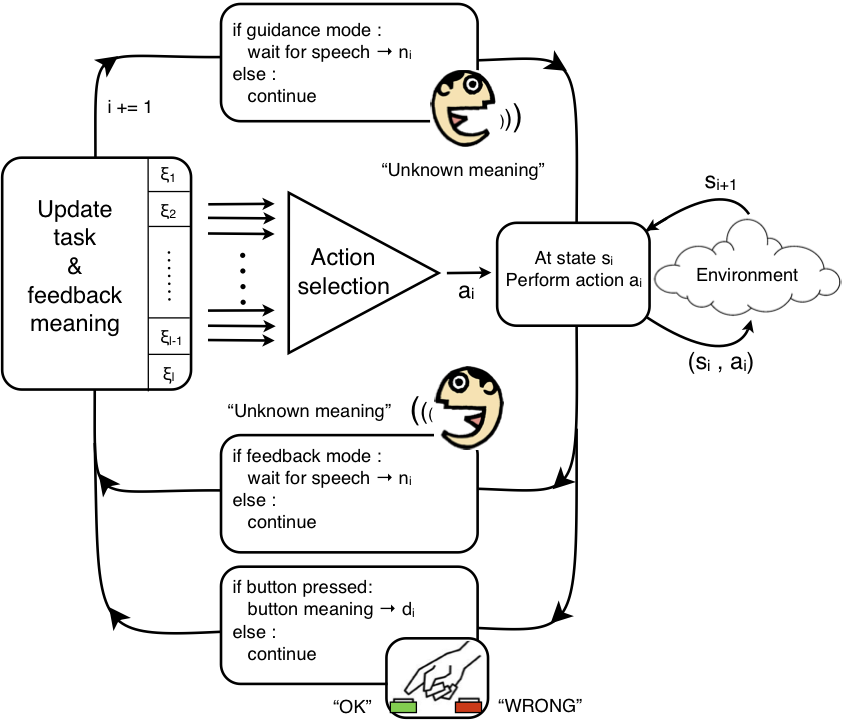
\includegraphics[width=\columnwidth]{images/bloc4.png}
	\caption{Experimental protocol showing the interaction between the teacher and the learning agent. The agent has to learn a task and the meaning of the instructions signals provided by the user, here recorded speech. The teacher can use guidance or feedback instructions but also has access to buttons of known meaning for the robot.}
	\label{bloc}	
\end{figure}
%
\subsubsection{Robotic System}
\label{sec:RoboticSystem}
%
We consider a six d.o.f. robotic arm and gripper that is able to grasp, transport and release cubes in four positions. We used a total of three cubes that can form towers of two cubes.  The robot has 4 actions available: \textit{rotate left}, \textit{rotate right}, \textit{grasp cube} and \textit{release cube}. The state space is discrete and defined as the location of each object, including being on top of another or in the robot's hand. So for a set of 3 objects we have 624 different states. Figure~\ref{setup} shows the robot grasping the orange cube. 
%
\begin{figure}[!htbp]
	\centering
		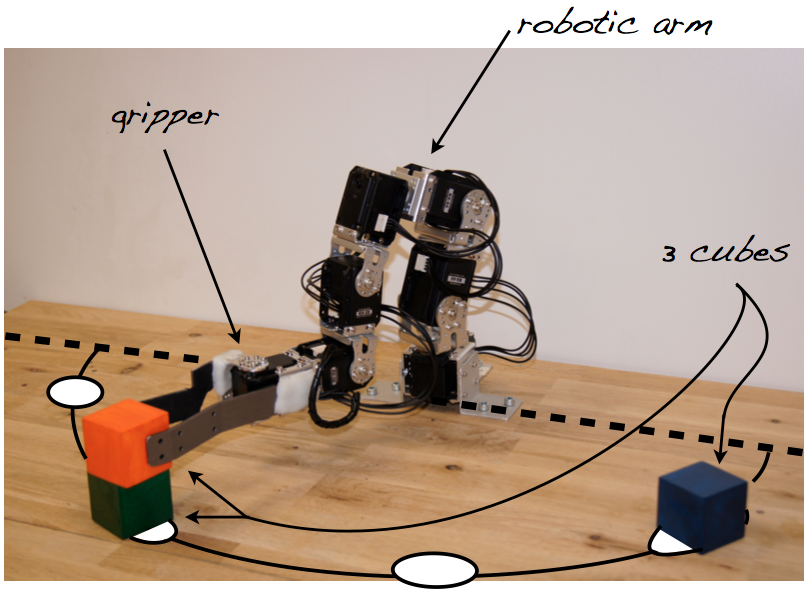
\includegraphics[width=0.8\columnwidth]{images/setup4.png}
	\caption{Robotic System. A six d.o.f robotic arm and gripper learning to perform a pick-and-place task with three cubes.
	        %An example of cubes' configuration which can be described as: \emph{"orange cube is on top of green cube in position 3, blue cube is in position 1 and the robot is grasping the orange cube"}.
	        }
	\label{setup}
\end{figure}
%
\subsubsection{Task Representation}
\label{sec:TaskRepresentation}
%
We assume that for a particular task $\xi$ we are able to compute a policy $\pi$ representing the optimal actions to perform in every state. One possibility is to use \textit{Markov Decision Processes} (MDP) to represent the problem \cite{sutton1998reinforcement}. From a given task $\xi$ represented as a reward function we can compute the corresponding policy using, for instance, \textit{Value Iteration} \cite{sutton1998reinforcement}. In any case, our algorithm does not make any assumption about how tasks are represented.

For this particular representation we assume that the reward function is sparse and so we can generate possible tasks by sampling sparse reward functions. Similarly to \textit{Bayesian Inverse Reinforcement Learning} \cite{Ramachandran07ijcai} the robot learns the task by choosing among the possible space of rewards the most likely one. We approximate this process using a finite set of task hypothesis representing all the reward functions consisting of a unitary reward in one state and no reward in all the others. In other words the task is to reach one, yet unknown, of the 624 states of the MDP.

Under this formalism the action selection at runtime can be done in different ways. As different sampling methods can lead to different learning behaviors, we will compare two different methods: random and  $\epsilon$-greedy. When following random action selection the robot does not use its current knowledge of the task and randomly selects actions. Whereas with $\epsilon$-greedy method the robot performs actions according to the current belief of what the task is, i.e. following the policy corresponding to the most likely task hypothesis. The corresponding optimal action is chosen with $1-\epsilon$ probability, otherwise, a random one is selected. In our experiment we show only results with $\epsilon =  0.1$.
%
%Indeed the quality of the samples received depends on the path the robot will follow in the MDP, some can lead to very informative feedback and others to a waste of time.
%
\subsubsection{Speech processing}
\label{sec:SpeechProcessing}
%
As mentioned before, we consider speech as the modality for interacting with the robot. After each action we record the teaching word pronounced by the user. This data is mapped into a $20$ dimensional feature space using the methodology described below.

A classical method for representing sounds is the \textit{Mel-Frequency Cepstral Coefficients} (MFCC) \cite{zheng2001comparison}. It represents a sound as a time sequence MFCC vectors of dimension $12$. Comparing sounds is done via \textit{Dynamic Time Warping} (DTW) between two sequences of feature vectors \cite{sakoe1978dynamic}. This distance is a measure of similarity that takes into account possible insertions and deletions in the feature sequence and is adapted for sounds comparison of different length. Each recorded vocal signal is represented as its DTW distance to a base of 20 pre-defined spoken words which are \textbf{not} part of words used by the teacher.

By empirical testing on recorded speech samples, we estimate that a number of 20 bases words were sufficient and yet a relatively high number of dimensions to deal with a variety of people and speech. This base of 20 spoken words has been randomly sampled from a scientific book\footnote{RA Wilson, FC Keil, "The MIT encyclopedia of cognitive science", 2001} and is composed of the words: \emph{ \footnotesize{Error, Acquisition, Difficulties, Semantic, Track, Computer, Explored, Distribution, Century, Reinforcement, Almost, Language, Alone, Kinds, Humans, Axons, Primitives, Vision, Nature, Building}}.
%
\subsubsection{Classification System for the Instruction Model}
\label{sec:classifiers}
%
As explained in Section \ref{sec:Algorithm}, any standard machine learning classifier can be used to approximate the instruction model. If such classifier is not able to use probabilistic labels then the maximization step of the EM algorithm is approximated in Eq. \ref{eq:F} with a hard thresholds for $z_{ij}^{\xi}$. We then have to rely on the generalization performances of the classifier. Indeed, if the classification algorithm is overfitting the data then no difference can be found between the hypotheses. The only required characteristic is the ability to output a confidence on the class prediction, i.e. a probability for $n_i$ of being associated to each meaning.

In this study we decided to compare three classifiers for the instruction learning, i.e. modeling $p(n|z,\theta)$:
\begin{itemize}
\item Gaussian Bayesian Classifier: Computing the weighted mean $\mu$ and covariance matrix $\Sigma$, the usual equations for gaussian mixture hold.
\item Support Vector Machine (SVM): Using a RBF kernel with $\sigma = 1000$ (high dimensional space) and $C = 0.1$.  For SVM probabilistic prediction refer to \cite{platt1999probabilistic}.
\item Logistic regression: The predictive output value ([0,1]) is used as a measure of confidence. This algorithm is usually not well suited for high dimensional spaces because of the curse of dimensionality.
\end{itemize}
%
\subsection{Experimental Results}
\label{sec:ExperimentalResults}
%
Experiments presented in this section follow the protocol described in figure~\ref{bloc}, where at each iteration the agent performs one action and waits for the instruction from the teacher. We first present a set of simulated experiments using the same MDP as for the real word experiment. We start by assuming that the teacher provides feedback instructions without any mistake, therefore only the variability in the signals remains. We first compare the different classifiers and then the performances of $\epsilon$-greedy versus random action selection methods both for feedback and guidance modes. Later, we present an analysis of robustness to teacher mistakes. Last simulated experiment studies the case where the teacher has also access to buttons of known meaning. Finally, we show results using a real robot where we study how instructions knowledge learned in a first run can be used in a second one to learn more efficiently.

%stay as close as possible to the real world setup, data used as teaching signals in simulation are recorded spoken words mapped to our 20 dimensional space. We remember that their everyday meaning have no relation with their meaning in the experiment, e.g. \emph{``Bad''} could be used to give a positive feedback. We recorded enough samples of each word to avoid using the same sample twice in the same run. Most of the results presented are from simulated experiments, however the simulated teacher is using real speech data recorded from a human and mapped to a fixed length feature vector as described in the following section~\ref{sec:SpeechProcessing}. This allow to test our system with realistic continuous features while controlling the behavior of teacher in terms of teaching mistake.
%Such words consist of:  \emph{\small{Good, Bad, Left, Right, Grasp, UnGrasp, Yes, No, Clockwise, CounterClockwise, Hold, PutDown}}, we remember that their everyday meaning have no relation with their meaning in the experiment, e.g. \emph{``Left''} could be used to give a positive feedback. We recorded enough samples of each word to avoid using the same sample twice in the same run.
%
In order to be able to compute statistically significant results for the learning algorithm, we created a database of speech signals that can be used in simulated experiments. This database allows to test our system with realistic continuous features while controlling the behavior of the teacher, e.g. by varying the amount teaching mistake. All results report averages of 20 executions of the algorithm with different start and goal states. By normalizing the sum of all likelihoods estimate ($q_1,\ldots,q_l$) to 1, we obtain the probability of each particular task hypothesis to represent the task to learn. The normalized likelihood of the task to be learned $q(\xi^*)$ is our measure of learning progress.
%
\subsubsection{Learning feedback instructions}
%
In this experiment we assume that the robot does not know the words being spoken by the teacher and it does not know the task either. The teacher is providing instruction of meaning being either \texttt{correct} or \texttt{wrong}. The robot will, simultaneously, learn the task and map the words that is recorded into a binary feedback signal.

The results comparing the different classification methods are shown in Figure~\ref{fig:FeedbackOneWord}. Action selection is done $\epsilon$-greedy. Note that after 200 iterations all three methods have learned the task, i.e. the normalized goal likelihood value is greater than 0.5, meaning that the sum of all the others is inferior to 0.5. Logistic regression provides the worse results in terms of convergence rate and variance.
%
\begin{figure}[!htbp]
	\centering
		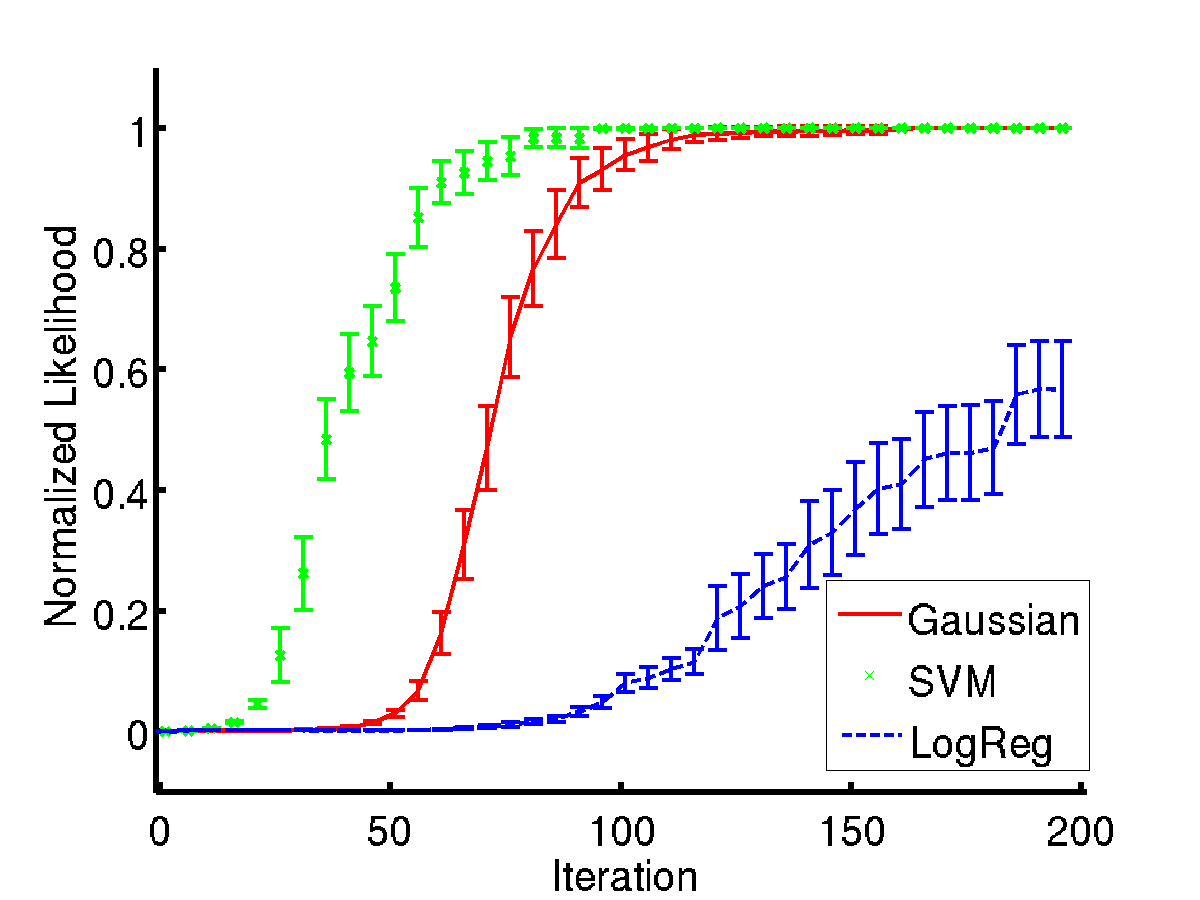
\includegraphics[width=\ww\columnwidth]{images/results/classifiers}
	\caption{Taught hypothesis normalized likelihood evolution (mean + std error) thought iteration using different kinds of classifiers. The teacher is providing feedback using one word per meaning and the agent is performing action according to $\epsilon$-greedy strategy.}
	\label{fig:FeedbackOneWord}
\end{figure}

The user is not restricted to the use of one word per meaning, table~\ref{tab:1} compares the goal normalized likelihood value after 100 iterations for feedback instructions composed of one, three and six spoken words per meaning. SVM has better performance when using one word per meaning but the Gaussian classifier has overall better results with less variance, see Table~\ref{tab:1}. 
%
\begin{table}[htbp]
\caption{Taught hypothesis normalized likelihood values after 100 iterations. Comparison for different classifiers and number of words per meaning. The gaussian classifier has overall better performances.}
\label{tab:1}
\centering
\begin{tabular}{|l|c|c|c|}
\hline
&\textbf{One word}&\textbf{Three words}&\textbf{Six words}\\\hline
\textbf{Gaussian}&1.0 (0.1)&1.0 (0.1)&0.7 (0.1)\\\hline
\textbf{SVM}&1.0 (0.0)&0.5 (0.4)&0.3 (0.4)\\\hline
\textbf{LogReg}&0.1 (0.1)&0.2 (0.3)&0.2 (0.3)\\\hline
\end{tabular}
\end{table}
%
Interestingly the Gaussian classifier learns better than the other classifiers with many words per meaning. This counter intuitive result can be explain by the high dimensionality of the space where even one gaussian can differentiate several group of clusters. As expected logistic regression performs badly due to the high dimensionality of the space. For the SVM classifier, the small number of points in each cluster is probably affecting the performances. For the following experiments, we will only consider the gaussian classifier, first because it has overall better performance but also because it is by far the faster to train and thus is the only one usable for real world and real time experiments. Indeed, in this setup, at each iteration the agent has to train 624 classifiers.
%
\begin{figure}[!htbp]
	\centering
		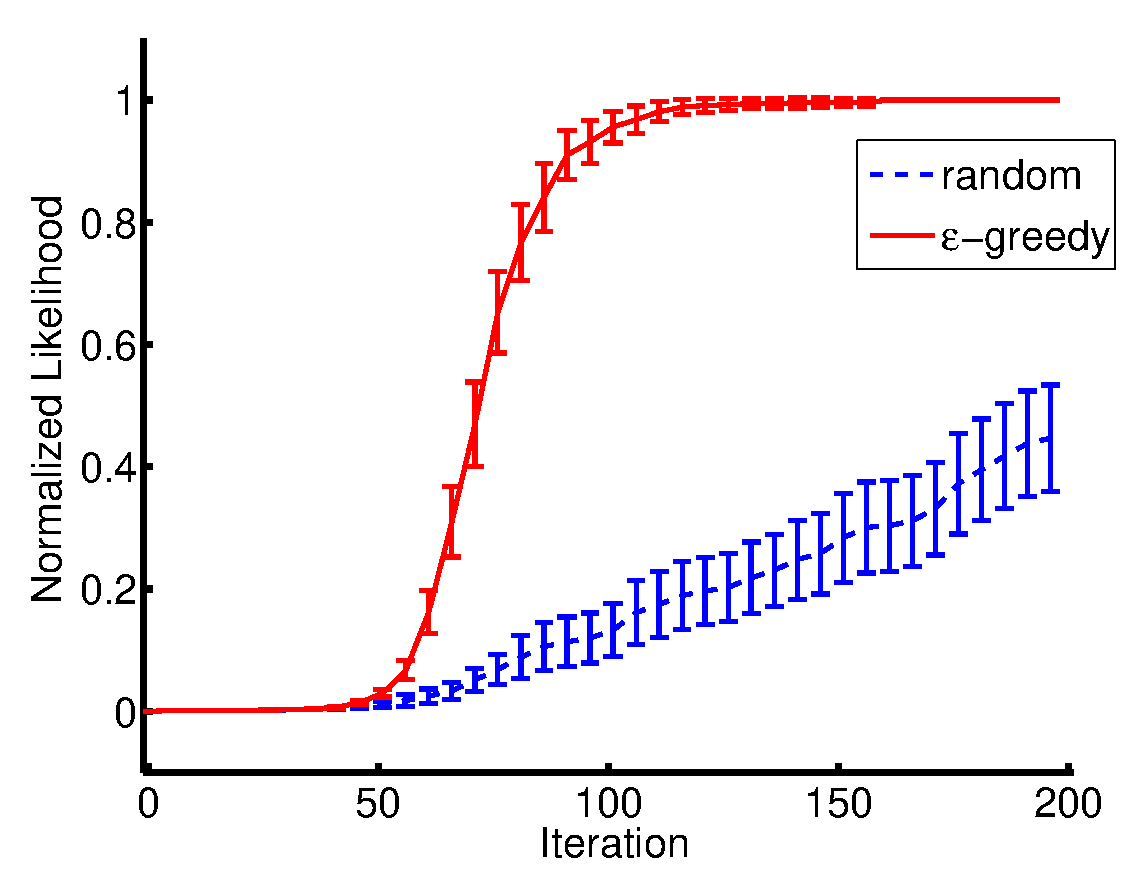
\includegraphics[width=\ww\columnwidth]{images/results/feedback}
	\caption{Taught hypothesis normalized likelihood evolution (mean + std error) thought iteration using gaussian classifier. The teacher is providing feedback using one word per meaning. The $\epsilon$-greedy action selection method learns faster than the random one. }
	\label{fig:FeedbackGaussianRdmGreed}
\end{figure}

We will now compare the impact of using different action selection methods. From Figure~\ref{fig:FeedbackGaussianRdmGreed} we can observe that $\epsilon$-greedy results in a faster learning with less variance. This method, at each step, leads the robot in the direction of the most probable goal.
In this way it will receive more diverse feedback and will visit more relevant states than what a simple random exploration would do.
%
\subsubsection{Learning guidance instructions}
%
Figure~\ref{fig:Guidance}, shows results where the teacher provides guidance instead of feedback. The number of meanings is increased from two (correct/wrong) to four (left/right/grasp/release). At each iteration the teacher first says the name of the optimal action to be performed by the robot, which then performs one action. Changes in the algorithm are described in Eq.~\ref{eq:likact}. As with feedback, the robot is able to learn the task based on guidance instructions but need more iterations to reach a perfect knowledge. Indeed, even if the robot receives more informative instructions, it now needs to classify instructions in four meanings which requires more samples to identify the clusters.  
%
\begin{figure}[!htbp]
	\centering
		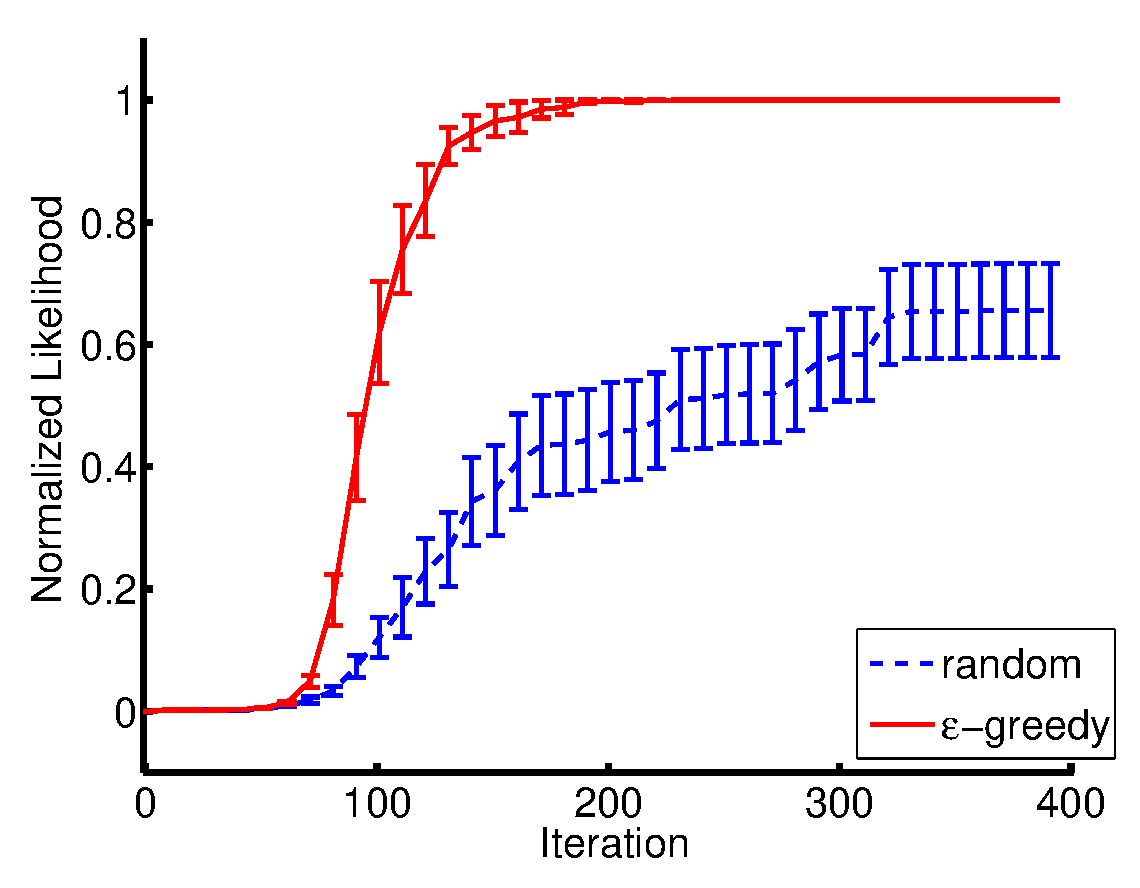
\includegraphics[width=\ww\columnwidth]{images/results/guidance}
	\caption{Taught hypothesis normalized likelihood evolution (mean + std error) thought iteration using gaussian classifier. The teacher is providing guidance using one word per action name. The $\epsilon$-greedy action selection method learns faster than the random one. }
	\label{fig:Guidance}
\end{figure}

\subsubsection{Robustness to teaching mistakes}

In results presented until now, we made the assumption that the teacher is providing feedback or guidance instructions without any mistake. But real world interactions are not perfect and people can fail in providing correct feedback. An analysis of robustness is shown in figure~\ref{fig:Noise} using feedback instructions, gaussian classifier and one word per meaning. Results with and without EM are compared to study if EM is improving robustness to teaching mistakes.
%
\begin{figure}[!htbp]
	\centering
		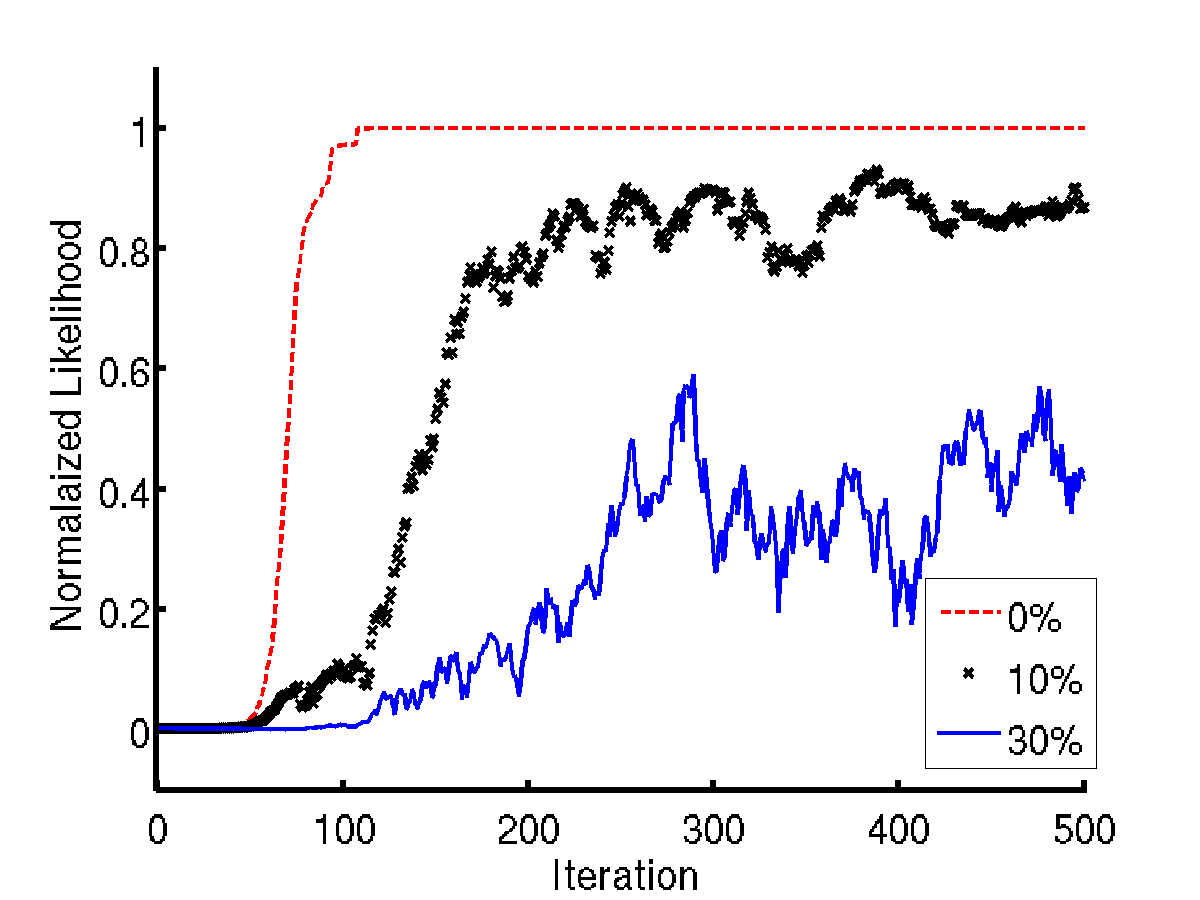
\includegraphics[width=\ww\columnwidth]{images/results/noise_no_EM}
		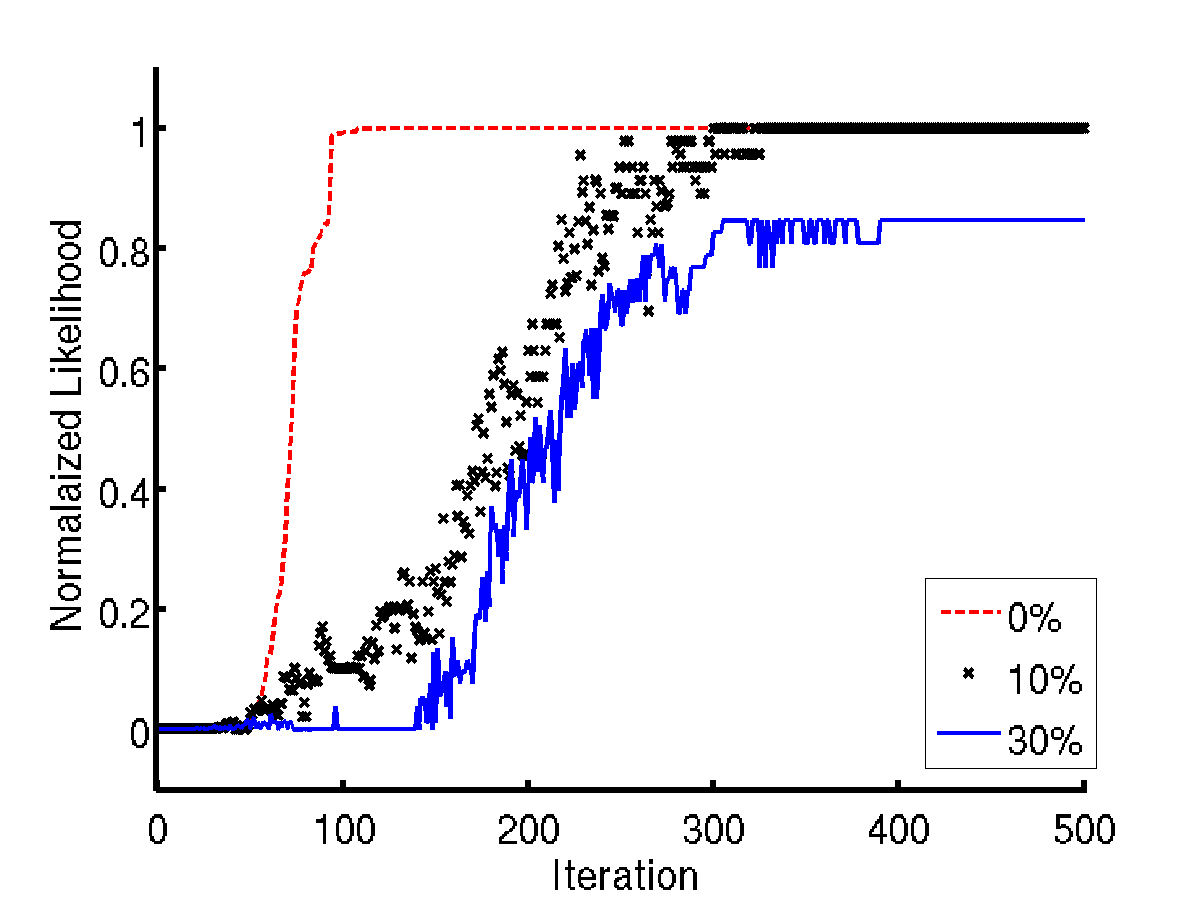
\includegraphics[width=\ww\columnwidth]{images/results/noise_with_EM}
	\caption{Taught hypothesis normalized likelihood evolution thought iteration using gaussian classifier. Comparison of one step EM (top) versus full EM (bottom). The teacher is providing feedback using one word per meaning with different percentage of mistakes. $\epsilon$-greedy action selection. Standard error has been omitted for readability reason. }
	\label{fig:Noise}
\end{figure}

We can observe that full EM is performing as expected and enables the agent to learn the task faster facing teaching mistakes. %The iterative process of EM will converge to the maximum likelihood parameters of our statistical model, reallocating teaching mistake
%Note that both technics should converge to 1 after some time.

\subsubsection{Including prior information}
\label{sec:IncludingPriorInformation}
%
Learning purely from unknown instructions is challenging for the researcher but could be restrictive for the teacher. Therefore sources of known feedback could be added, such as a green and red button, where the green button has a predefined association with a \texttt{correct} feedback meaning, as red button with a \texttt{wrong} meaning. Yet, we shall expect that even in this case, users will use more modalities than the predefined one. 
%For example, in some experiments with a robot that is explained not being capable of hearing, a majority of people are still talking to the robot \cite{rouanet2013impact}. 
In this study, the teacher still provides initially unknown spoken words feedback but can also use the red and green button as described in figure~\ref{bloc}. However, and in order to avoid possibility of direct button to instruction association, it can never use both modalities at the same time and use them alternatively with equal probability. 
%This allows us to constrain the experiment in cases where a direct mapping from button to unknown signals could not be used. 
Therefore, in average after 250 iterations the robot has received 125 known feedback and 125 unknown speech signals. This setting assumes that more information is received by the robot than the one predefined by the developer. In most systems this information is ignored but we think robots could also try learning from such unknown signals. We study three learning methods: in the first case, the robot is learning only via the known feedback, i.e. the buttons; in the second it uses only the vocal unknown signal; and in the third one, it uses both.  Figure~\ref{fig:button} shows result from this setting. 
%
\begin{figure}[!htbp]
	\centering
		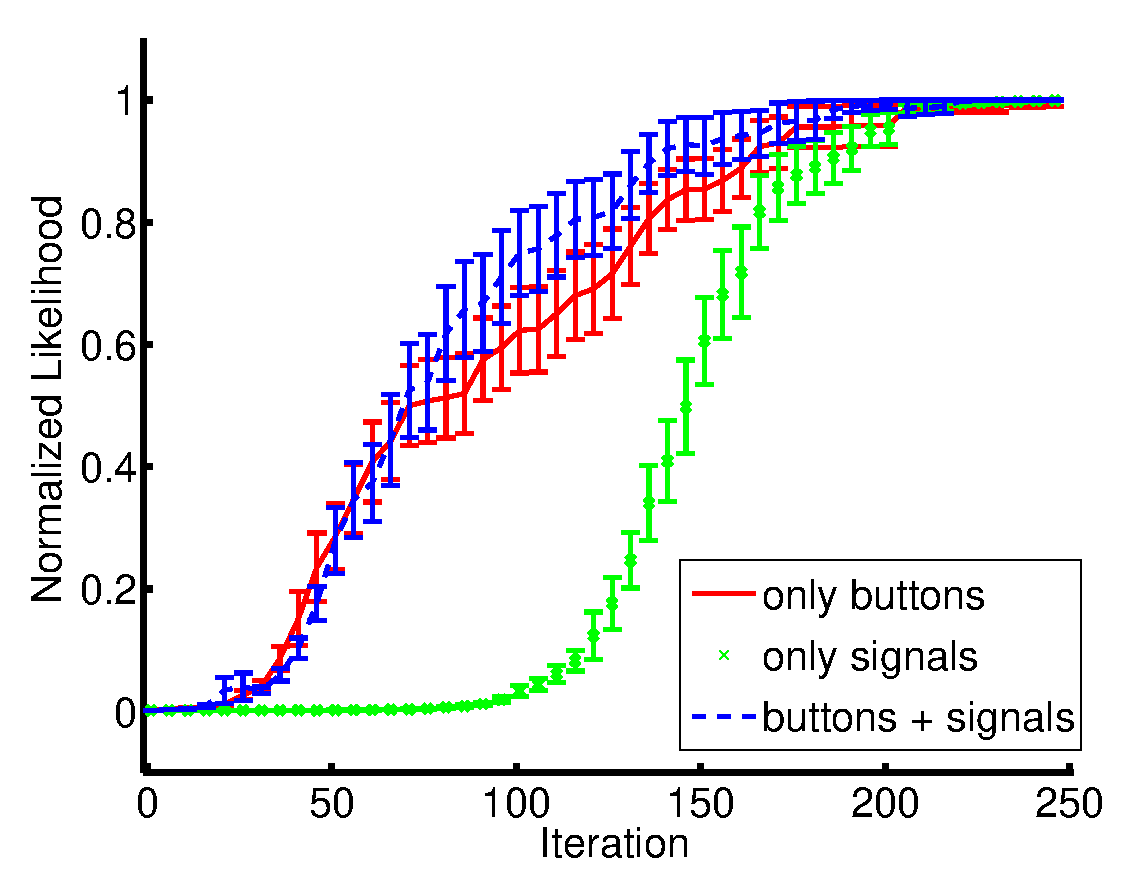
\includegraphics[width=\ww\columnwidth]{images/results/mix_button}
	\caption{Taught hypothesis normalized likelihood evolution (mean + std error) thought iteration using gaussian classifier. Comparison of using known, unknown signals and both.}
	\label{fig:button}
\end{figure}

As expected learning from known feedback is faster than with unknown, however taking advantage of different sources of information, even a priori unknown, can lead to slightly better performances than using only known information. Importantly, the instructions to meaning knowledge of the robot is updated and could therefore be reuse in further interaction.

\subsubsection{Using a real robot}
%
Statistical simulations have shown that our algorithm allows an agent to learn a task from unknown feedback in a limited amount of interactions. To bridge the gap of simulation we tested our algorithm in real interaction condition with our robotic arm. In this real experiment, the teacher is facing the robot and chooses a specific goal to reach (i.e. a specific arrangement of cube it wants the robot to build). It then decides one word to use as positive feedback and one as negative feedback and starts to teach the robot. For this experiment the word \textit{'yes'} and \textit{'no'} were respectively used for the meaning \texttt{correct} and \texttt{wrong}. Once this  experiment is terminated we keep in memory the classifier corresponding to the best task, i.e. having the higher likelihood value, and start a new experiment where the human teacher is going to use the same feedback instructions to teach a new task. But this time the spoken words are first classified as of correct or wrong meaning according to the previously learnt classifier. Therefore standard IRL algorithm can be used. We study here two things, first does our system bridges the reality gap and can we reuse information learnt from a previous experience? 
%
\begin{figure}[!htbp]
	\centering
		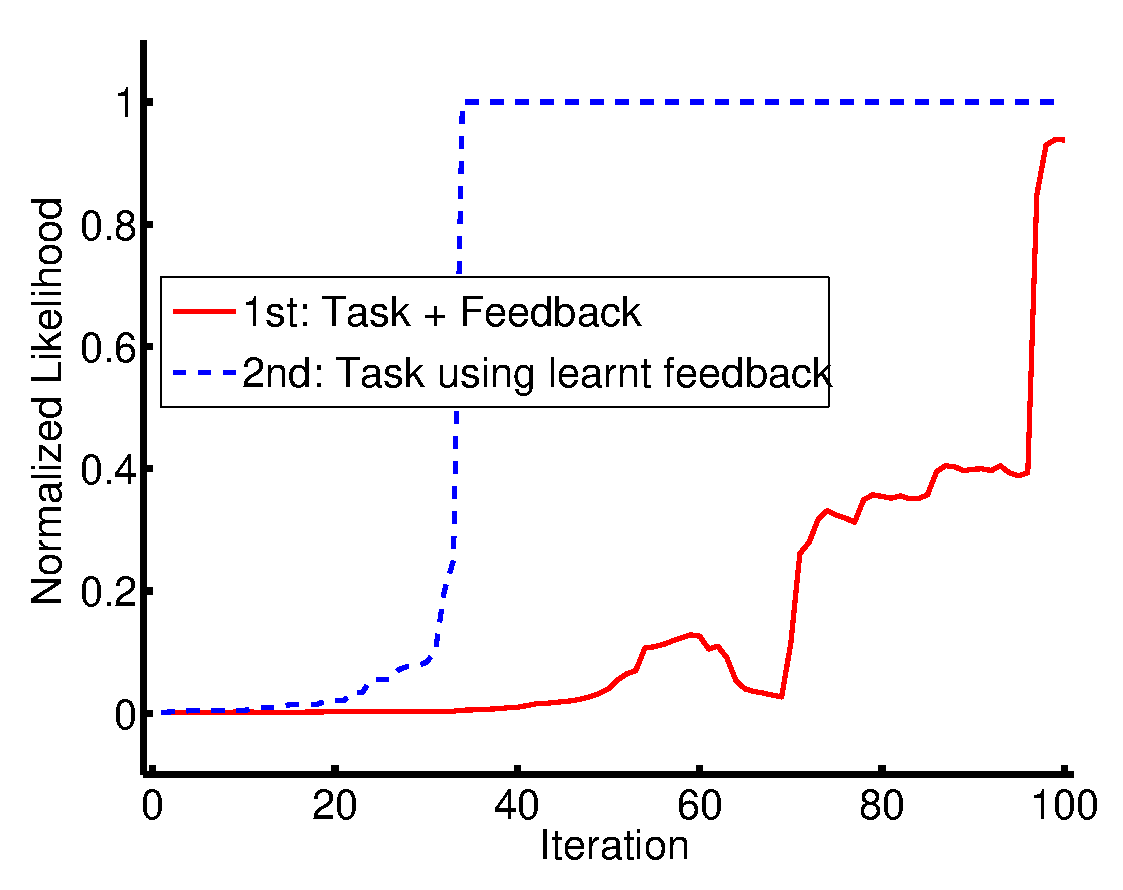
\includegraphics[width=\ww\columnwidth]{images/results/real}
	\caption{Taught hypothesis normalized likelihood evolution thought iteration using gaussian classifier.  Feedback using one word per action. $\epsilon$-greedy action selection. A first run of 100 iterations is performed where the robot learns a task from unknown feedback. Then by freezing the classifier corresponding to the best task estimate, the user teaches the robot a new task.}
	\label{Real}
\end{figure}

Figure~\ref{Real} shows results from this setting. In the first run it takes about 100 iterations for the robot to learn the task. Whereas in the second run, when reusing knowledge from the first one, the robot is able to learn a new task faster, in about 30 iterations, meaning that it has well found the two clusters in our $\mathbb{R}^{20}$ dimensional space as well as the mapping to their corresponding meanings.

%\footnote{A video explaining this experiment can be found at : \small{\url{http://flowers.inria.fr/learning-unknown-feedback.mp4}}}

\begin{comment}
\section{Results}
\label{sec:Results}

 In this section we present results from our algorithm both in simulation and with a real robotic system where we test different aspects: a) learning the associated meaning of teaching words while learning a new task, b) extend it for the case of guidance words, c) combine learning from unknown signals with pre-defined signals of known meanings, d) reuse learnt signals to meaning association for the learning of a new task.

\subsection{Experimental System}
\label{sec:ExperimentalSetup}

We construct a small size pick-and-place task with a real robot. This robot is going to be programmed using a natural language interface whose words have an unknown meaning. The robot has a prior knowledge about the distribution of possible tasks and knows how to accept teaching signals.

The interaction between the robot and the human is forced to be a turn taking social behavior, where the robot is performing an action and wait for a feedback or guidance signal to continue. This allows us to synchronize a vocal word to the corresponding pair of state and action. The experimental protocol is summarized in figure~\ref{bloc}.

\begin{figure}[!htbp]
	\centering
		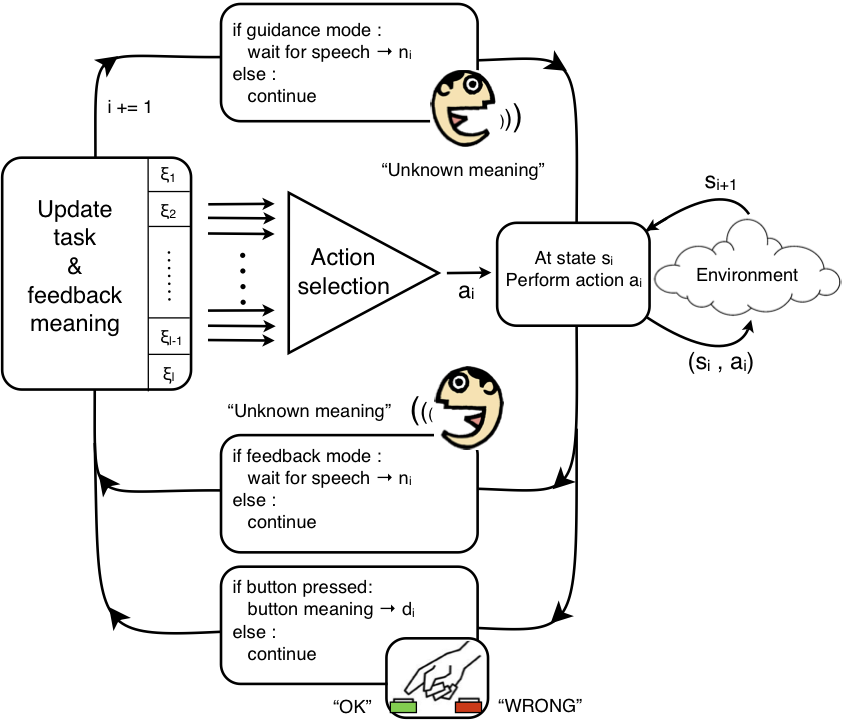
\includegraphics[width=0.9\columnwidth]{images/bloc4.png}
	\caption{Experimental protocol showing the interaction between the teacher and the learning agent. The agent has to learn a task and the meaning of the signals provided by the user, here recorded speech. The teacher can use guidance or feedback signals but has also access to buttons of known meaning for the robot.\vspace{-0.1cm}}
	\label{bloc}
	
\end{figure}

\subsubsection{Robotic System}
\label{sec:RoboticSystem}
%
We consider a six d.o.f. robotic arm and gripper that is able to grasp, transport and release cubes in four discrete positions. We used a total of three cubes that can form towers of at most two cubes.  The robot has 4 actions available: \textit{rotate left}, \textit{rotate right}, \textit{grasp cube} and \textit{release cube}. The state space is discrete and defined as the location of each object, including being on top of another or in the robot's hand. So for a set of 3 objects we have 624 different states. Figure~\ref{setup} shows the robot grasping the orange cube. The system is open loop and if a cube is moved without ``informing'' the robot, it will fail executing its plan. 

\begin{figure}[!htbp]
	\centering
		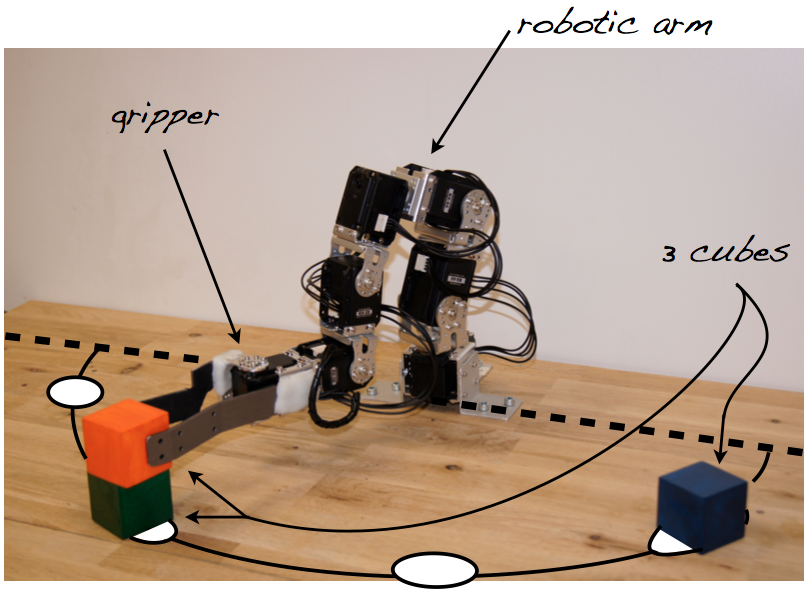
\includegraphics[width=0.6\columnwidth]{images/setup4.png}
	\caption{Robotic System. An example of cubes configuration which can be described as: \emph{
"orange cube is on top of green cube in position 3, blue cube is in position 1 and the robot is grasping the orange cube"}.\vspace{-0.5cm}}
	\label{setup}
\end{figure}

\subsubsection{Task Representation}
\label{sec:TaskRepresentation}

We assume that for a particular task $\xi$ we are able to compute a policy $\pi$ representing the optimal actions to perform in every state. One possibility is to use \textit{Markov Decision Processes} (MDP) to represent the problem \cite{sutton1998reinforcement}. From a given task $\xi$ represented as a reward function we can compute the corresponding policy using, for instance, Value Iteration. In any case, our algorithm does not make any assumption about how tasks are represented.

For this particular representation we assume that the reward function is sparse and so we can generate possible tasks by sampling sparse reward functions. Similarly to Bayesian Inverse Reinforcement Learning \cite{Ramachandran07ijcai} the robot learns the task by choosing among the possible space of rewards the most likely one. We approximate this process using a finite set of task hypothesis representing all the reward functions consisting of a unitary reward in one state and no reward in all the other. In other words the task is to reach one, yet unknown, of the 624 states of the MDP.

Under this formalism the action selection at runtime can be done in different ways. As different sampling methods can lead to different learning behaviors we will compare two different methods: random and  $\epsilon$-greedy. When following random action selection the robot does not use its current knowledge of the task and randomly select actions. Whereas with $\epsilon$-greedy method the robot performs actions according to the current belief of what the task is, i.e. following the policy corresponding to the most likely task hypothesis. The corresponding optimal action is chosen with $\epsilon$ probability, otherwise, a random one is selected. In our experiment we show only results with $\epsilon =  0.9$.

%Indeed the quality of the samples received depends on the path the robot will follow in the MDP, some can lead to very informative feedback and others to a waste of time.

\subsubsection{Speech processing}
\label{sec:SpeechProcessing}

As mentioned before, we consider speech as the modality for interacting with the robot. After each action we record the teaching word pronounced by the user. This data is mapped into a $20$ dimensional feature space using the methodology described next.  

A classical method for representing sounds is the \textit{Mel-Frequency Cepstral Coefficients} (MFCC) \cite{zheng2001comparison}. It represents a sound as a time sequence of features vector, called MFCC coefficient. Feature vector dimension can vary, in our case we used 12. Comparing sounds can then be done via \textit{Dynamic Time Warping} (DTW) between two sequences of feature vectors \cite{sakoe1978dynamic}. This distance is a measure of similarity that takes into account possible insertions and deletions in the feature sequence and is adapted for sounds comparison of different length. Each recorded vocal signal is represented as its DTW distance to 20 pre-defined base of spoken words.

By empirical test on recorded speech samples, we estimate that a number of 20 bases words were sufficient and yet a relatively high number of dimensions to deal with a variety of people and speech. This base of 20 words have been randomly selected and is composed of the words:\emph{ \footnotesize{Error, Acquisition, Difficulties, Semantic, Track, Computer, Explored, Distribution, Century, Reinforcement, Almost, Language, Alone, Kinds, Humans, Axons, Primitives, Vision, Nature, Building}}.

\subsubsection{Classification System for the Symbol Model}
\label{sec:classifiers}

As explained in section \ref{sec:Algorithm}, any standard machine learning classifier can be used for approximating the symbol model. If such classifier is not able to use probabilistic labels then the maximization step of the EM algorithm is approximated in Eq. \ref{eq:F} with a hard thresholds for $z_i^{\xi}$. We then have to rely on the generalization performances of the classifier. Indeed, if the classification algorithm is overfitting the data then no differences can be found between the different hypotheses. The only required characteristic is the ability to output a confidence on the class prediction, i.e. a probability for $n_i$ of being associated to each meaning.

In this study we decided to compare three classifiers for the symbol learning:
\begin{itemize}
\item Gaussian Bayesian Classifier: Computing the weighted mean $\mu$ and covariance matrix $\Sigma$, the usual equations for gaussian mixture hold.
\item Support Vector Machine (SVM): Using a RBF kernel with $\sigma = 1000$ (high dimensional space) and $C = 0.1$.  For SVM probabilistic prediction refer to \cite{platt1999probabilistic}.
\item Logistic regression: The predictive output value ($\in [0,1]$) is used as a measure of confidence. This algorithm is usually not well suited for high dimensional spaces as the euclidean distances are huge in such spaces.
\end{itemize}

\subsection{Experimental Results}
\label{sec:ExperimentalResults}

Experiments presented in this section follow the protocol described in figure~\ref{bloc}, where by turn the agent perform one action and wait for teaching signals from the teacher. Teacher is providing a signal after each action of the robot. We first present a set of statistical simulated experiments using the same MDP as for the real word experiment. We start by assuming that the teacher is providing feedback without any mistake, therefore only the noise in the signals remain. We compare first the different classifiers, and then the performances of $\epsilon$-greedy versus random action selection methods both for feedback and guidance mode. Later, we present an analysis of robustness to teacher mistakes while comparing one step EM with full EM. Last simulated experiment studies the case where the teacher has also access to buttons of known meaning. Finally, we show the result of one real word experiment where we study how signals knowledge learnt in a first run can be used in a second one to learn more efficiently.

In order to stay as close as possible to the real world setup, data used as teaching signals in simulation are recorded spoken words mapped to our 20 dimensional space. Such words consist of:  \emph{\small{Good, Bad, Left, Right, Grasp, UnGrasp, Yes, No, Clockwise, CounterClockwise, Hold, PutDown}}, we remember that their everyday meaning have no relation with their meaning in the experiment, e.g. \emph{``Left''} could be used to give a positive feedback. We recorded enough samples of each word to avoid using the same sample twice in the same run.

All results report averages of 20 executions of the algorithm with different start and goal states. By normalizing the sum of all likelihoods estimate ($q_1,\ldots,q_l$) to 1, we obtain the probability of each particular task hypothesis to represent the task to learn. The normalized likelihood of the task to be learnt $q(\xi^*)$ is our measure of learning progress.

\subsubsection{Learning feedback signals}

In this experiment we assume that the robot does not know the words being spoken by the teacher and it does not know the task either. The robot will, simultaneously, learn the task and map the words that is recording into a binary feedback signal.

The results comparing the different classification methods are shown in Figure~\ref{fig:FeedbackOneWord}. Action selection is done $\epsilon$-greedy. Note that after 200 iterations all three methods learn the task, i.e. the normalized goal likelihood value is greater than 0.5, meaning that the sum of all the others is inferior to 0.5. Logistic regression provides the worse results in terms of convergence rate and variance. \vspace{-0.3cm}

\begin{figure}[!htbp]
	\centering
		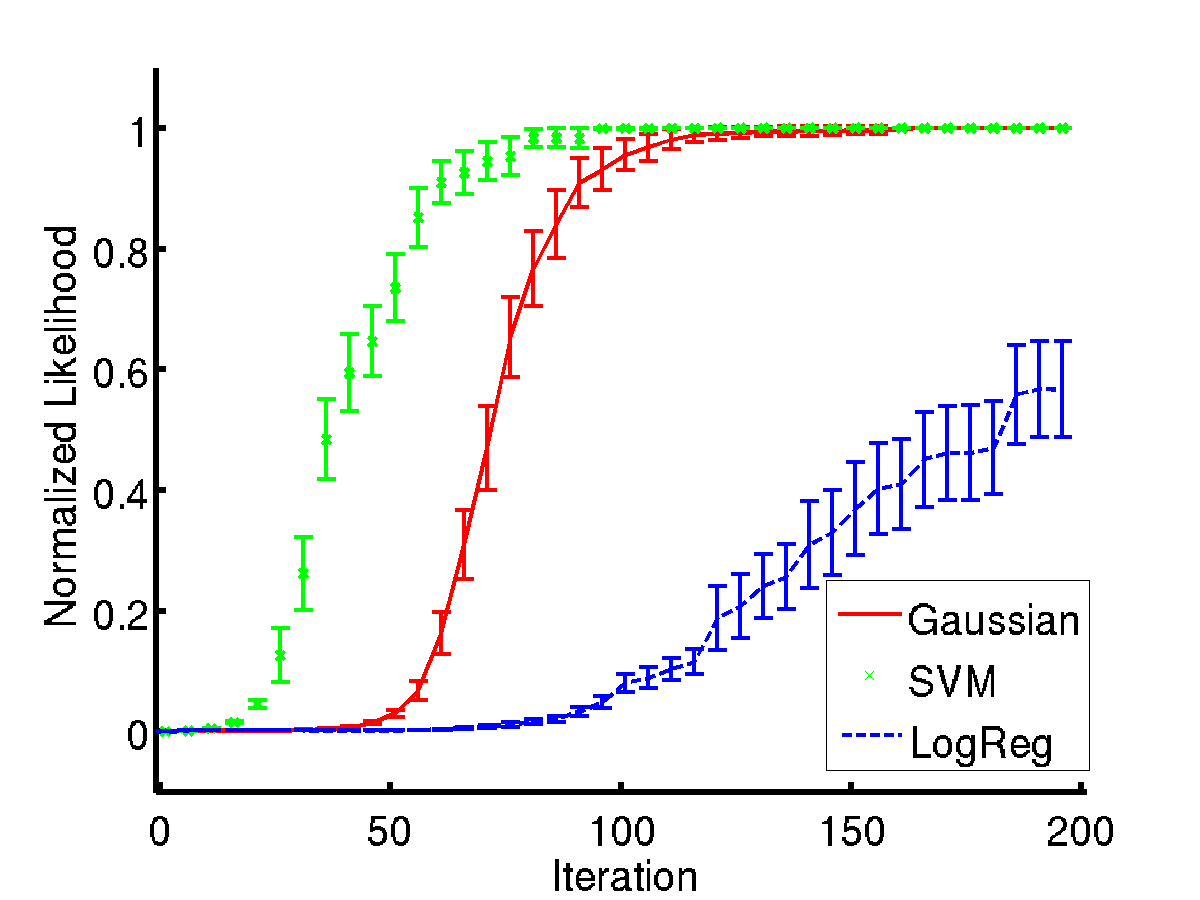
\includegraphics[width=\ww\columnwidth]{images/results/classifiers}
	\caption{Goal normalized likelihood evolution (mean + std error) thought iteration using different kinds of classifiers. The teacher is providing feedback using one word per meaning and the agent is performing action according to $\epsilon$-greedy method. \vspace{-0.1cm} }
	\label{fig:FeedbackOneWord}
\end{figure}

The user is not restricted to the use of one word per meaning, table~\ref{tab:1} compares the goal normalized likelihood value after 100 iterations for feedback signals composed of one, three and six spoken words per meaning. SVM has better performance when using one word per meaning but the Gaussian classifier has overall better results with less variance, see Table~\ref{tab:1}. 

\begin{table}[htbp]
\caption{\scriptsize{Mean and variance goal normalized likelihood values after 100 iterations. Comparison for different classifiers and number of words per meaning. The gaussian classifier has overall better performances.}}
\label{tab:1}
\centering
\begin{tabular}{|l|c|c|c|}
\hline
&\textbf{One word}&\textbf{Three words}&\textbf{Six words}\\\hline
\textbf{Gaussian}&1.0 (0.1)&1.0 (0.1)&0.7 (0.1)\\\hline
\textbf{SVM}&1.0 (0.0)&0.5 (0.4)&0.3 (0.4)\\\hline
\textbf{LogReg}&0.1 (0.1)&0.2 (0.3)&0.2 (0.3)\\\hline
\end{tabular}

\end{table}

Interestingly the Gaussian classifier learns better than the other classifiers with many words per meaning. This counter intuitive result can be explain by the high dimensionality of the space where even one gaussian can differentiate several group of clusters. As expected logistic regression performs badly due to the high dimensionality of the space. For the SVM classifier, the small number of points in each cluster is probably affecting the performances. For following experiments, we will only consider the gaussian classifier, first because it has overall better performance but also because it is by far the faster to train and thus is the only one usable for real world and real time experiments. Indeed, in this setup, at each iteration the agent has to train 624 classifiers.\vspace{-0.2cm}

\begin{figure}[!htbp]
	\centering
		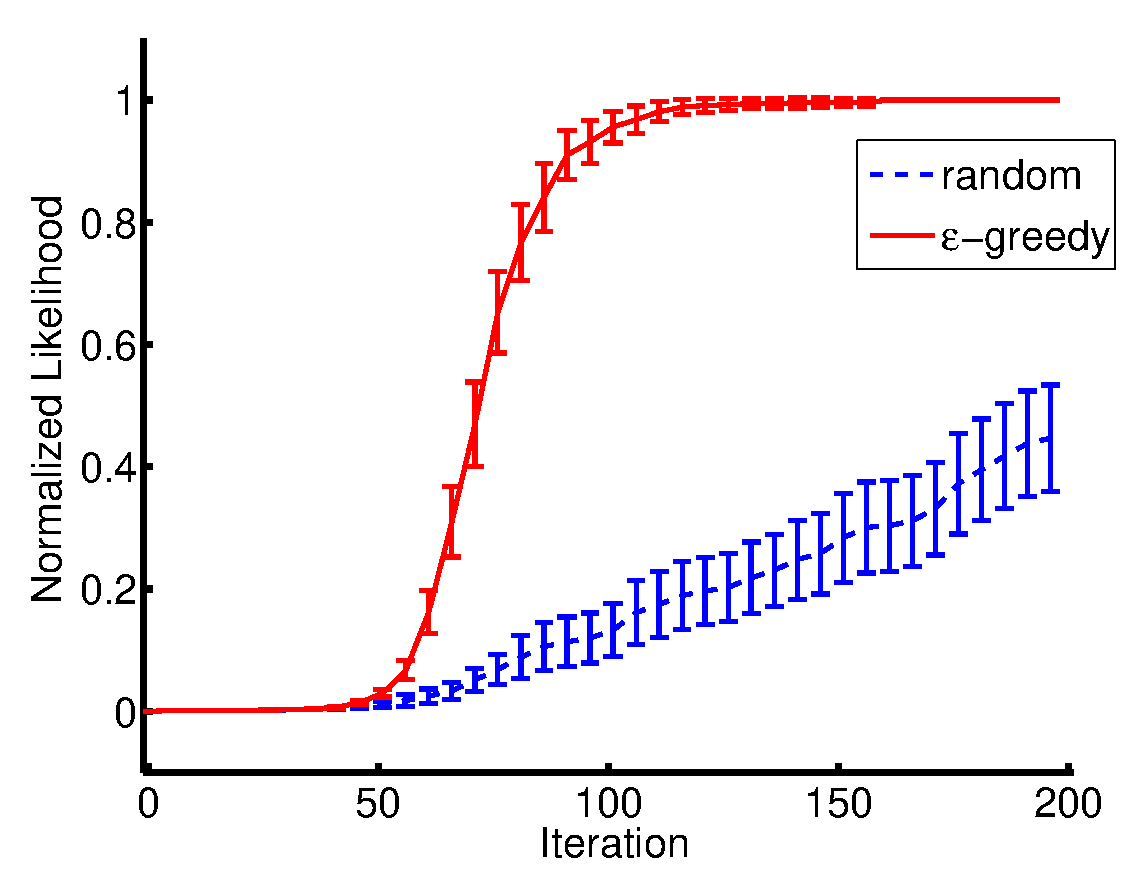
\includegraphics[width=\ww\columnwidth]{images/results/feedback}
	\caption{Goal normalized likelihood evolution (mean + std error) thought iteration using gaussian classifier. The teacher is providing feedback using one word per meaning. The $\epsilon$-greedy action selection method learns faster than the random one. \vspace{-0.2cm}}
	\label{fig:FeedbackGaussianRdmGreed}
\end{figure}

We will now compare the impact of using different action selection methods. From Figure~\ref{fig:FeedbackGaussianRdmGreed} we can observe that $\epsilon$-greedy results in a faster learning with less variance. This method, at each step, leads the robot in the direction of the most probable goal.
In this way it will receive more diverse feedback and will visit more relevant states than what a simple random exploration would do.

\subsubsection{Learning guidance signals}

Figure~\ref{fig:FeedbackOneWord}, shows results where the teacher provides guidance instead of feedback. The number of meaning is increased from two (correct/wrong) to four (left/right/grasp/release). At each iteration the teacher first says the name of the optimal action to be performed by the robot, which then performs one action. Changes in the algorithm are described in Eq.~\ref{eq:likact}. As with feedback, the robot is able to learn the task based on guidance signals but need more iterations to reach a perfect knowledge. Even if the robot receives more informative signals, it now needs to classify them in four different meanings which requires more samples. \vspace{-0.1cm}

\begin{figure}[!htbp]
	\centering
		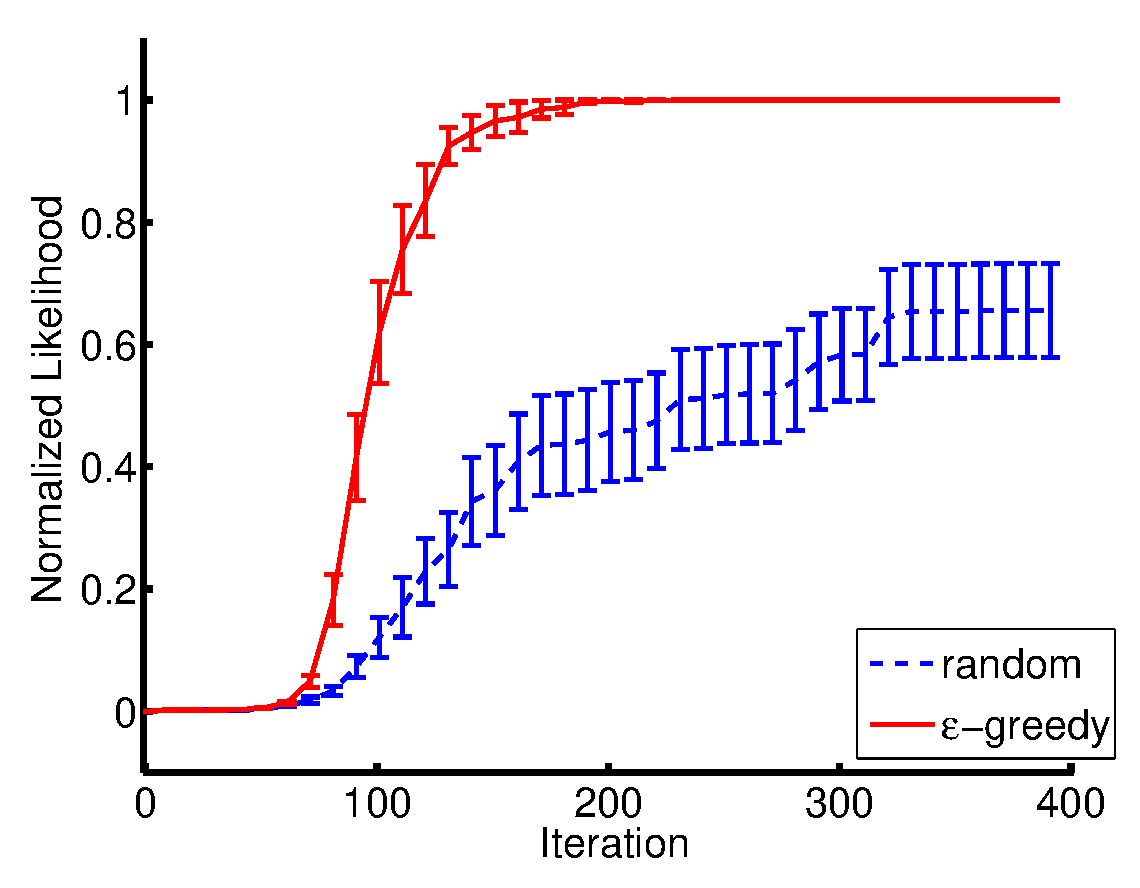
\includegraphics[width=\ww\columnwidth]{images/results/guidance}
	\caption{Goal normalized likelihood evolution (mean + std error) thought iteration using gaussian classifier. The teacher is providing guidance using one word per action name. The $\epsilon$-greedy action selection method learns faster than the random one. \vspace{-0.1cm}}
	\label{fig:Guidance}
\end{figure}

\subsubsection{Robustness to teaching mistake}

In results presented until now, we made the assumption that the teacher is providing feedback or guidance signals without any mistake. But real world interactions are not perfect and people can fail in providing correct feedback. An analysis of robustness is shown in figure~\ref{fig:Noise} using feedback signals, gaussian classifier and one word per meaning. Results with one step EM and full EM are compared to study if  full EM is improving robustness to teaching mistakes. \vspace{-0.2cm}

\begin{figure}[!htbp]
	\centering
		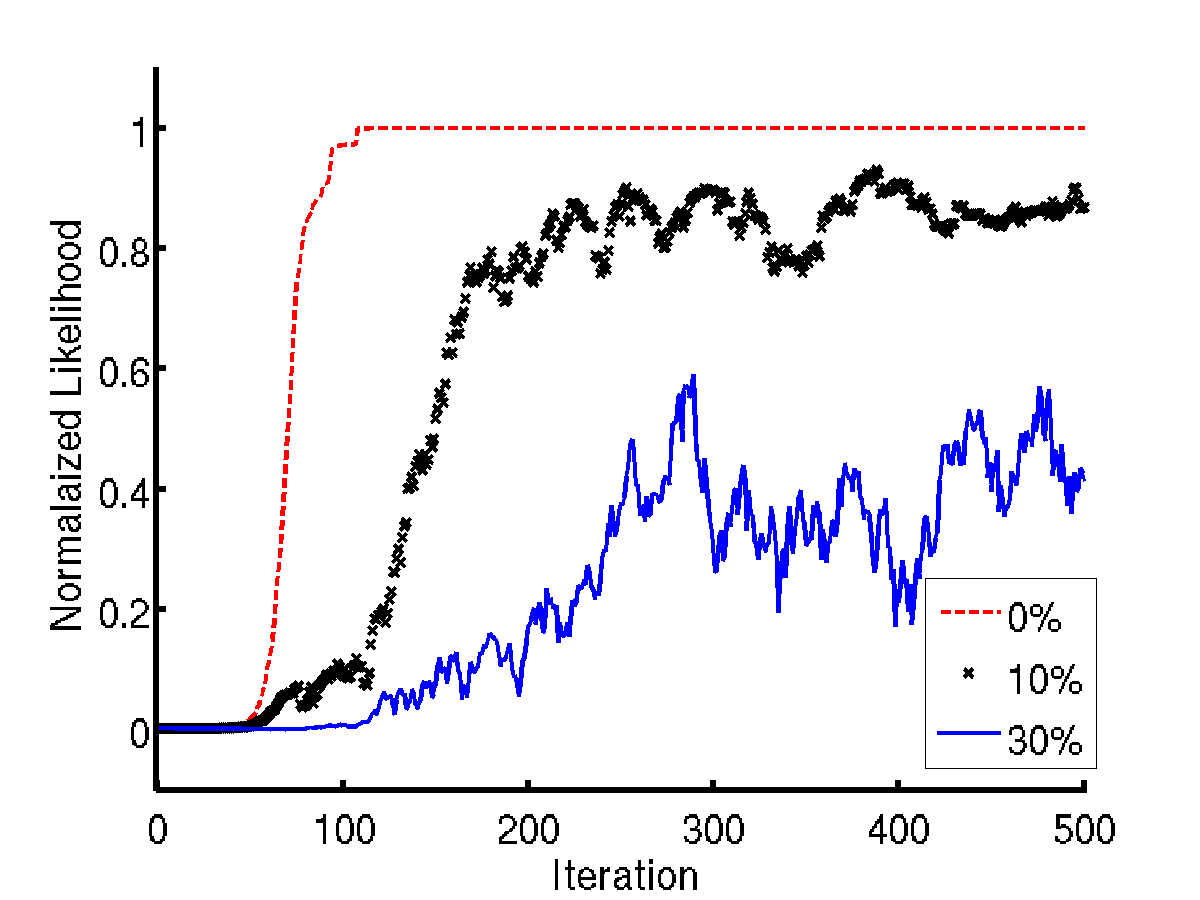
\includegraphics[width=0.60\columnwidth]{images/results/noise_no_EM}
		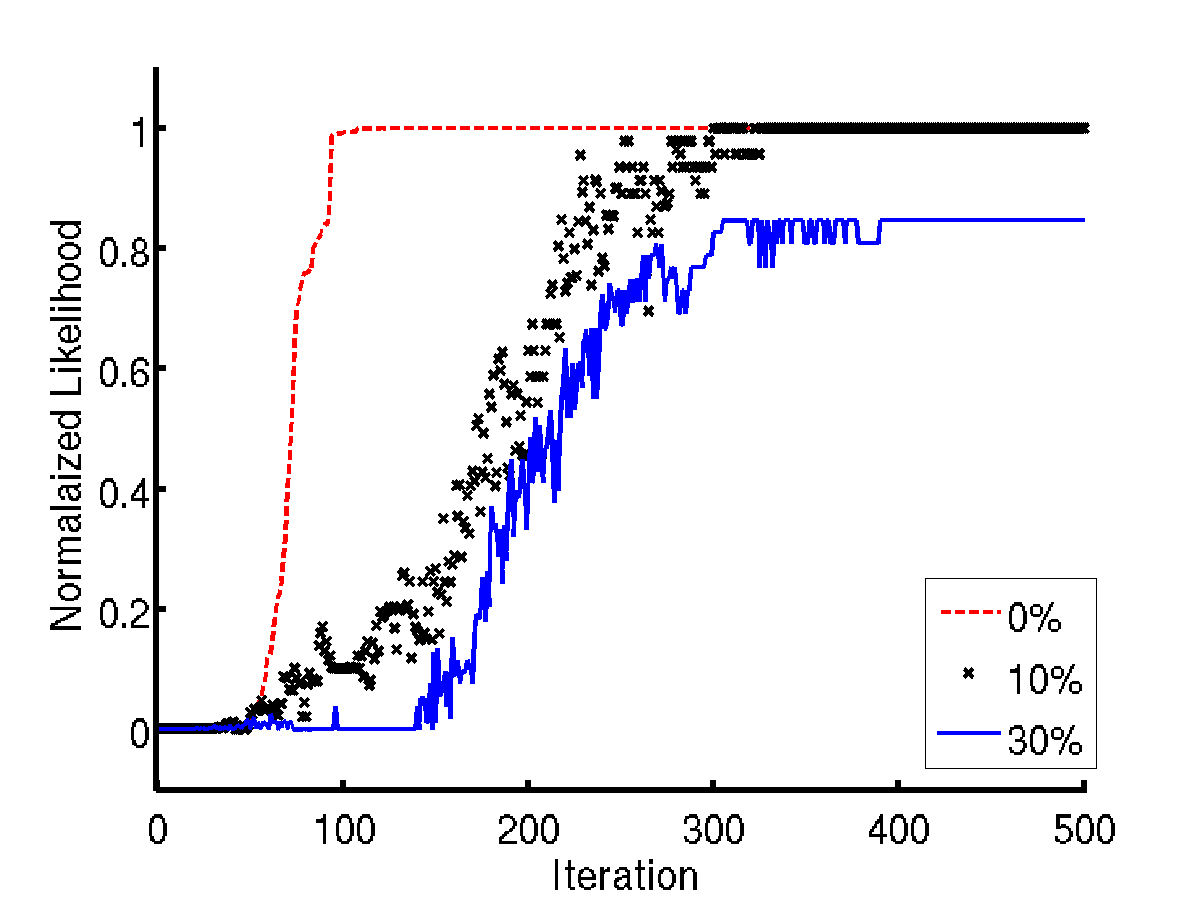
\includegraphics[width=0.60\columnwidth]{images/results/noise_with_EM}
	\caption{Goal normalized likelihood evolution thought iteration using gaussian classifier. Comparison of one step EM (top) versus full EM (bottom). The teacher is providing feedback using one word per meaning with different percentage of mistake. $\epsilon$-greedy action selection. Standard error has been omitted for readability reason. \vspace{-0.4cm}}
	\label{fig:Noise}
\end{figure}

We can observe that full EM is performing as expected and enables the agent to learn the task faster facing teaching mistake.
%Note that both technics should converge to 1 after some time.

\subsubsection{Including prior information}
\label{sec:IncludingPriorInformation}

Learning purely from unknown teaching signals is challenging for the researcher but could be restrictive for the teacher. Therefore sources of known feedback could be added, such as a green and red button. Where the green button has a predefined association with a \texttt{correct} feedback meaning, as red button with a \texttt{wrong} meaning. Yet, we shall expect that even in this case, users will use more modalities than the predefined one. 
%For example, in some experiments with a robot that is explained not being capable of hearing, a majority of people are still talking to the robot \cite{rouanet2013impact}. 
In this study, the teacher still provides initially unknown spoken words feedback but can also use the red and green button as described in figure~\ref{bloc}. However, and in order to avoid possibility of direct button to signal association, it can never use both modalities at the same time and use them alternatively with equal probability. 
%This allows us to constrain the experiment in cases where a direct mapping from button to unknown signals could not be used. 
Therefore, in average after 250 iterations the robot has received 125 known feedback and 125 unknown speech signals. This setting assumes that more information is received by the robot than the one predefined by the developer. In most systems this information is ignored but we think robots could also try learning from such unknow signals. We study three learning methods: in the first case, the robot is learning only via the known feedback, i.e. the buttons; in the second it uses only the vocal unknown signal; and in the third one, it uses both.  Figure~\ref{fig:button} shows result from this setting. \vspace{-0.2cm}

\begin{figure}[!htbp]
	\centering
		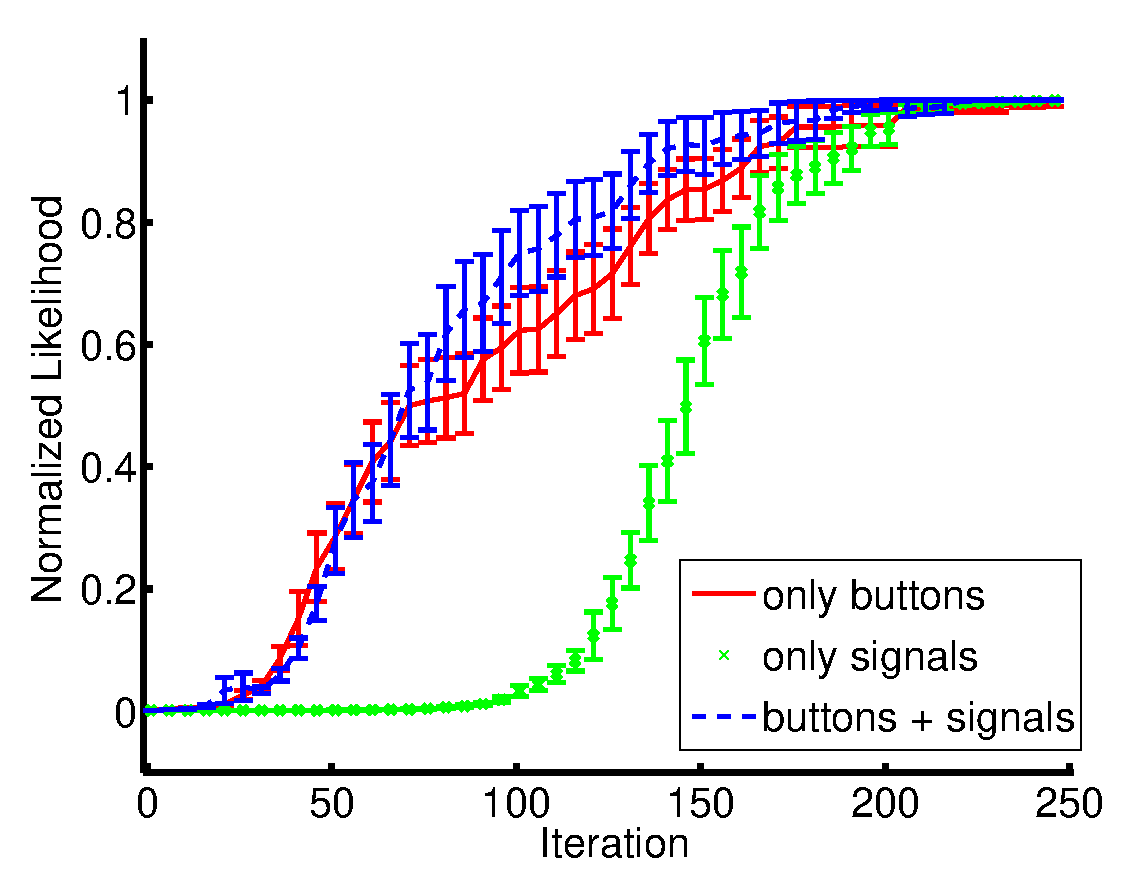
\includegraphics[width=\ww\columnwidth]{images/results/mix_button}
	\caption{Goal normalized likelihood evolution (mean + std error) thought iteration using gaussian classifier. Comparison of using known, unknown signals and both. Standard deviation have been omitted for readability.\vspace{-0.1cm}}
	\label{fig:button}
\end{figure}

As expected learning from known feedback is faster than with unknown, however taking advantage of different sources of information, even a priori unknown, can led to slightly better performances than using only known information. Importantly, the signals to meaning knowledge of the robot is updated and could therefore be reuse in further interaction.

\subsubsection{A real word experiment}

Statistical simulations have shown that our algorithm allows an agent to learn a task from unknown feedback in a limited amount of interactions. To bridge the gap of simulation we tested our algorithm in real interaction condition with our robotic arm. In this real experiment, the teacher is facing the robot and chooses a specific goal to reach (i.e. a specific arrangement of cube he wants the robot to build). He then decides one word to use as positive feedback and one as negative feedback and starts to teach the robot. Once this  experiment is terminated we keep in memory the classifier corresponding to the best task, i.e. having the higher likelihood value, and start a new experiment where the human teacher is going to use the same feedback signals to teach a new task. But this time the spoken words are first classified as of correct or wrong meaning according to the previously learnt classifier. Therefore standard IRL algorithm can be used. We study here two things, first does our system bridges the reality gap and can we reuse information learnt from a previous experience? 

\begin{figure}[!htbp]
	\centering
		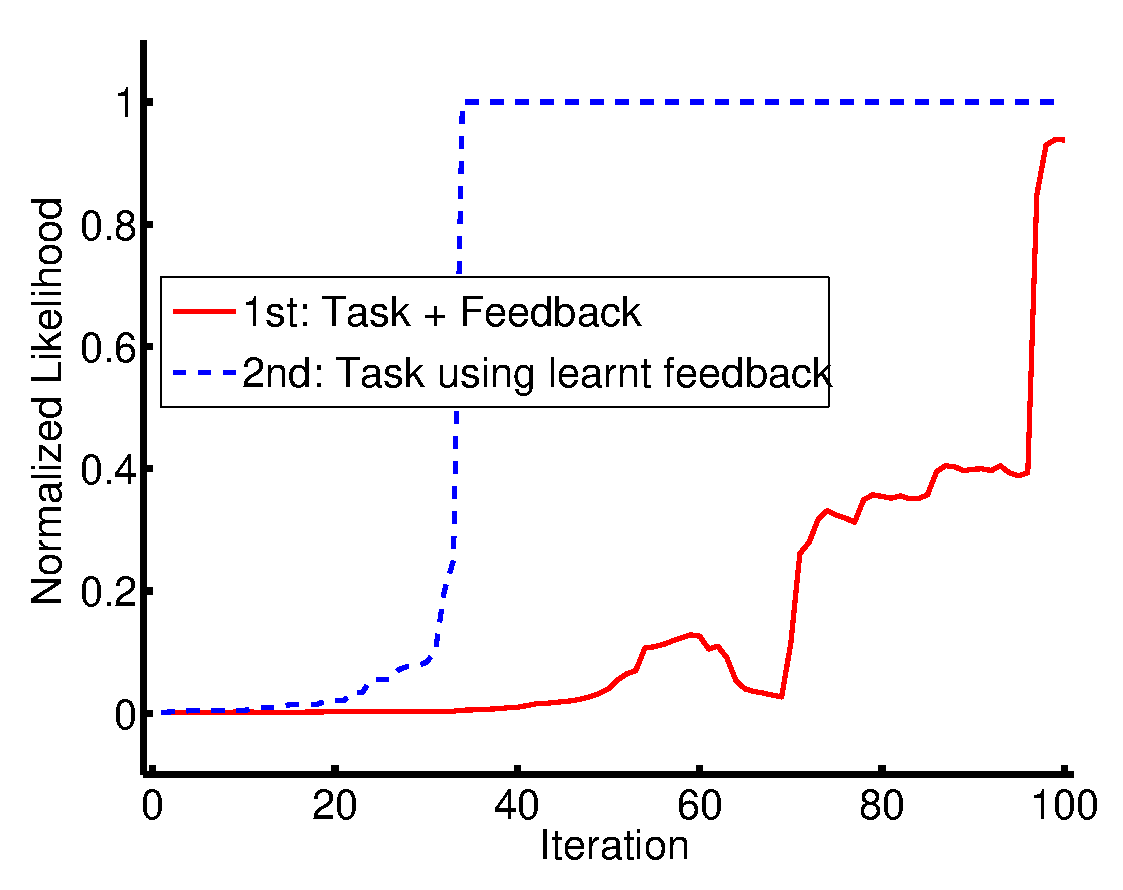
\includegraphics[width=\ww\columnwidth]{images/results/real}
	\caption{Goal normalized likelihood evolution thought iteration using gaussian classifier.  Feedback using one word per action. $\epsilon$-greedy action selection. A first run of 100 iterations is performed where the robot learns a task from unknown feedback. Then by freezing the classifier corresponding to the best task estimate, the user teaches the robot a new task.\vspace{-0.5cm}}
	\label{Real}
\end{figure}

Figure~\ref{Real} shows results from this setting. In the first run it takes about 100 iterations for the robot to learn the task. Whereas in the second run, when reusing knowledge from the first one, the robot is able to learn a new task faster, in about 30 iterations, meaning that it has well found the two clusters in our $\mathbb{R}^{20}$ dimensional space as well as the mapping to their corresponding meanings.

%\footnote{A video explaining the all process can be found at : \small{\url{http://flowers.inria.fr/learning-unknown-feedback.mpg}}}

\end{comment}

\section{Conclusions, Limitations And Future Work}
\label{sec:LimitationAndFutureWork}
%
In this work, we presented an interactive learning system that can learn the meaning of instructions while learning a new task. We considered the case of spoken words but of particular interest is the possibility to use the same system with other modalities, such as facial expressions or hand gestures. This allows different users to use the system according to their own preferences, skills, and limitations. We tested our experiment on a real robot and showed that knowledge acquired from a first experiment can be reused later as a source of known information. 

Our approach assumes that the robot is equipped with planning skills and can not be used if several hypothesis are fully symmetric as they will not be distinguishable. This problem can be solved by redefining the set of hypothesis, for instance by adding a ''stop'' action valid only at the goal states. 

In order to make the learning problem tractable, we assumed that the robot had access to a predefined set of tasks. The robot will then find the hypothesis that best approximates the true one. We could extend this and follow a particle filter like approach to be able to generate new hypothesis online and potentially find a better one.

%The current work is a starting point and some assumptions have been included. The interaction protocol is constrained to be turn taking and the possible meanings are limited to feedback or guidance on the robot's action.
%
In the future we will study how to extend the proposed approach to more complex scenarios, e.g. how it scales to continuous domain. We will also consider how more complex instructions can be included in our formalism since the teaching models used spontaneously by people can be more complex than the simple meaning correspondences we assumed \cite{Thomaz2008,Cakmak2010}. Also the protocol could be enhanced to be more natural, the robot could ask questions \cite{cakmak2012designing} and accept asynchronous signals. An important aspect is to allow the user to teach the robot new macro-actions or macro-states and a first approach for that problem is to use the options framework \cite{sutton1999between}.
%
%
%\section{Conclusions}
%In this work we presented an interactive learning system that can learn a task from unknown and noisy teaching signals while simultaneously estimating the associated meaning of such natural language utterances. 
%In this work we presented an interactive learning system that can learn the meaning of teaching signals while learning a new skill. We considered the case of spoken words but of particular interest is the possibility to use the same system with other modalities, such as facial expressions or hand gestures. 
%A robot that interacts repeatedly with the same teacher will be able to reuse part of its knowledge about the used teaching signals when acquiring new tasks.
%Our algorithm is an \textit{Expectation-Maximization} approach where the hidden variables are the true meanings of the words provided by the teacher. The algorithm is able to learn in this setting due to some assumptions about the class of problems that the robot is able to acquire and by finding the pairs of meaning-task that are more ``coherent'' in a statistical setting. The meanings are learned with standard classification algorithms where the best results are achieved with a simple gaussian classifier.
%We considered how the policy of the robot influences learning and observed that if the robot acts according to its current estimate of what the optimal policy is, the learning rate is higher. We studied two cases: a) the teacher provides feedback signals, i.e. a binary reward signal and b) the teacher provides guidance signals, i.e. an instruction of what the optimal action is. The algorithm works in both situations.
%Although we took such a difficult challenge of learning without assuming knowledge of the teaching signals, for a practical case it is more reasonable to combine pre-specified words with an adaptation to new words. This allows different users to use the system according to their own preferences, skills and limitations. The use of those extra sources of information is straightforward in our statistical formalism. 
%The main advantage of combining all the sources of information into the same algorithm is that mistakes in the teaching, e.g. the user presses the wrong button, can be corrected accurately. We observed that even with $30\%$ of errors in the feedback the system can identify the correct task with low uncertainty.
%Finally we tested our experiment in a real world implementation and showed that knowledge acquired from a first experiment can be reused later as a source of known information. A robot that interacts repeatedly with the same teacher will be able to reuse part of its knowledge about the used teaching signals when acquiring new tasks.
%
\section*{Acknowledgement}
The authors would like to thanks Pierre Rouanet for his useful comments, as well as J\'er\^{o}me Bechu for his help with the robotic platform. Work (partially) supported by INRIA, Conseil R\'egional d'Aquitaine and the ERC grant EXPLORERS 24007.

%### IEEE ###
\bibliographystyle{IEEEtran}
\bibliography{complete,macl,newref}



\end{document}